\section{Overview}
\label{sec:appendix_overview}
This supplementary material presents additional results to complement the main manuscript. 
First, we provide all the implementation details, including network architectures in~\cref{sec:details}.
Next, we elaborate on training details, such as the FoV sampling and datasets in~\cref{sec:training_details}.
Then, we describe how we perform class-agnostic instance segmentation in~\cref{sec:class_agnostic}.
Finally, we provide more qualitative comparisons on both video object tracking and class-agnostic instance segmentation in~\cref{sec:more_qualitative}.
% In addition to this document, we provide an interactive HTML interface to compare our video results with state-of-the-art methods.
In addition to this document, we provide additional video results to compare with state-of-the-art methods.


\section{Implementation Details} \label{sec:details}
Through all experiments, we use SAM~2.1-Large as our baseline due to computational resource constraints. A Hiera~\cite{ryali2023hiera} image encoder produces multi-scale features, where stride-16 and stride-32 outputs (Stages 3/4) are fused via an FPN~\cite{lin2017featureFPN} with convolutions to obtain frame embeddings, while shallow features (stride 4/8) from Stages 1/2 are injected only into the mask decoder to recover fine boundaries. Memory attention uses sinusoidal absolute positional embeddings together with 2D RoPE; object pointer tokens do not use RoPE, and we adopt $L=4$ layers. The prompt encoder follows SAM, and the mask decoder uses the mask token as the object pointer stored in the memory bank. An additional token predicts object visibility via an MLP head, and occluded frames receive a learned occlusion embedding in memory. As in SAM~2, the decoder outputs multiple mask candidates and selects the one with the highest predicted IoU when ambiguity persists. The memory encoder reuses Hiera features without a separate backbone; memory features are projected to 64 dimensions, and the 256-dim pointer is split into four 64-d tokens for cross-attention. For multi-object videos, the image encoder is shared while each object maintains an independent memory bank and decoder.
 
\subsection{Feature Merger}

% As illustrated in \cref{fig:feature-merging}, we use multi-layer feature from must3r decoder. 
% Note that we maintain MUSt3R's memory as it is, i.e. we do that alter the memory selection mechanism in MUSt3R, which is essentirally select by maximizing view coverage. The $[\text{encoder feature},4,7,11]$ layer index is selected empirically, as we want to introduce both semantic-aware(from early layers) and geometry-aware(from late layers, as it decodes point clouds from linear layer after the final transformer layer in must3r decoder, and we will also use the output point cloud).  After selecting the must3r features, we next merge it the cross attention layers. Specifically, we first gatther the positional embedding to following merging. The positional embedding is obtained by passing through the point map and ray map from must3r output, and we call this PE3D. PE2D is obtained by using Must3r's positional embedding. During merging, We first pass encoder feature through a conv layer to reduce dim from 1024 to 768, add PE3D, and then pass through a self attention layer with PE2D, which is called $F_{coarse}$. For the following $i\in [4, 7, 11]$, we update the $F_{coarse}$ by Attention layers, i.e. $F_{coarse}=FFN(CrossAttn(SelfAttn(F_{coarse}+PE3D), F_i+PE3D)$. We omit the normalization and skip connection for simplicity. After these attention blocks, we next pass $F_{coarse}$ through interplation and convolution layers and then concatenate with $F_{2D}$ from the SAM Image encoder, which is then refined by a convolution block to align the feature dims with $F_{2D}$. The final feature $F_{merged}$ is used as main feature for memory attention and memory encoding. Note that the shallow featrues from Hiera from Stages 1/2 are left untouched so that we can use such visual feature for fine mask output in mask decoder.

As illustrated in \cref{fig:feature-merging}, our method uses multi-layer features from the MUSt3R decoder.  
We keep MUSt3R’s memory mechanism unchanged—i.e., we do not modify its view-coverage–based memory selection.  
We empirically select the layer indices $[\text{encoder}, 4, 7, 11]$ to incorporate both semantic cues from early layers and geometry-aware signals from later layers, as deeper decoder layers in MUSt3R increasingly capture 3D structure and directly decode point clouds.

After selecting the MUSt3R features, we merge them using a sequence of cross-attention operations.  
We first construct positional embeddings: PE3D is obtained by processing the point map and ray map produced by MUSt3R, while PE2D is taken from MUSt3R’s 2D positional encoding.  
The encoder feature is projected from 1024 to 768 channels using a $1\!\times\!1$ convolution, added with PE3D, and then passed through a self-attention layer with PE2D to form an initial coarse feature $F_{\text{coarse}}$.

For each selected MUSt3R layer $F_i$ with $i \in \{4,7,11\}$, we update $F_{\text{coarse}}$ using:
\begin{equation} \small
\resizebox{\columnwidth}{!}{$
F_{\text{coarse}}
\leftarrow
\mathrm{FFN}\!\left(
\mathrm{CrossAttn}\!\big(
\mathrm{SelfAttn}(F_{\text{coarse}} + \mathrm{PE3D}),
\, F_i + \mathrm{PE3D}
\big)\right).
$}
\end{equation}
We omit normalization and skip connections for clarity.

After the attention fusion, $F_{\text{coarse}}$ is upsampled and refined by a $3\!\times\!3$ convolution, then concatenated with the Hiera image-encoder feature $F_{2D}$ from SAM~2, followed by an additional convolution block to match the feature dimensions.  
The resulting feature $F_{\text{merged}}$ is used for memory attention and memory encoding.  
We leave the shallow Hiera features from Stages~1 and~2 untouched so that the mask decoder can still rely on strong low-level visual cues for producing high-resolution segmentation outputs.


\section{Training Details} \label{sec:training_details}
\subsection{Field-of-View Sampling}
We do not use 100\% FOV-aware sampling because we observe that applying FOV filtering to every batch degrades the model’s original feature-matching ability inherited from SAM2.  
When all training samples come from drastically different viewpoints, the model is over-regularized toward cross-view matching and loses its within-view correspondence skills, leading to a form of feature collapse.  
% We therefore mix FOV-aware and continuous sampling, and analyze different sampling ratios in \cref{tab:sampling-ratio}.



% \begin{table}[t]
% \centering
% \caption{\textbf{Video Object Segmentation results between different sampling ratio on ScanNet++ Selected Set.} 
% Positive IoU is computed over frames with ground-truth masks. 
% Successful IoU is computed over frames where a ground-truth object exists and the IoU of prediction and GT $\neq 0$.}
% \label{tab:sampling-ratio}
% \resizebox{\columnwidth}{!}{
% \begin{tabular}{lccc}
% \toprule
% Method / FoV-aware Sampling Prob. & IoU $\uparrow$ & Positive IoU $\uparrow$ & Successful IoU $\uparrow$ \\
% \midrule
% Vanilla SAM2 / - & 0.3397 & 0.0179 & 0.0395 \\
% 3AM / 0.0 & 0.6945 & 0.4781 & 0.5024 \\
% 3AM / 0.8 & 0.9061 & 0.7168 & 0.7737 \\
% 3AM / 1.0 & 0.5811 & 0.3576 & 0.3913 \\
% \bottomrule
% \end{tabular}
% }
% \end{table}
\subsection{Settings}

\paragraph{Loss}
We follow SAM2's loss design without modification.  
Specifically, mask prediction is supervised using a weighted combination of focal loss (20) and dice loss (1);  
the IoU head is trained with an $\ell_{1}$ loss (1);  
and the occlusion prediction head uses a cross-entropy loss (1).

\paragraph{Prompts}
Due to the degraded 2D mask and the large viewpoint variations introduced by the sampling strategy during training, we restrict the input modality to masks only for ScanNet++ and ASE. For MOSE, we enable all prompt types, including point, box, and mask inputs.

\subsection{Datasets}
\paragraph{Aria Synthetic Environments (ASE)~\cite{avetisyan2024scenescript}}
ASE is a large-scale synthetic dataset of 100,000 procedurally generated indoor scenes rendered with simulated Aria-glass sensors. Each scene contains realistic 3D object layouts, simulated trajectories, and aligned 2D/3D annotations.
ASE enables large-scale training of 3D scene understanding, object detection, and tracking, particularly in data-hungry settings where real-world labelled data is scarce. 
We sample a total of 2{,}612 scenes whose number of views falls within a practical range:  
scenes with too few views do not provide sufficient viewpoint variation for training,  
while scenes with excessively many views lead to memory overflow when running MUSt3R. 

\paragraph{MOSE~\cite{MOSE}}
The MOSE dataset (Complex Video Object Segmentation) targets video-object segmentation in cluttered and occluded real-world scenes. It comprises 2,149 video clips with 5,200 objects from 36 categories and 431,725 high-quality masks.  
Unlike previous VOS benchmarks that feature large, salient, isolated targets, MOSE features heavy occlusion, object disappearance and re-appearance, and small/inconspicuous objects.
MOSE is primarily used to preserve the core VOS capability of our model.  
While our geometric integration encourages strong cross-view consistency, we do not want the model to over-rely on geometry and ``hallucinate'' object tracks without sufficient visual evidence; MOSE helps anchor the model to appearance-driven cues.  

Although MUSt3R supports dynamic scenes, we find that training on highly dynamic and diverse datasets such as SA-V Train leads to instability in practice. MOSE provides a more controlled level of motion and scene variation, allowing us to maintain stable learning while still leveraging dynamic-object supervision.


\paragraph{ScanNet++~\cite{yeshwanth2023scannet++}}
ScanNet++ is a high-quality indoor RGB--D reconstruction dataset that provides accurate camera poses, dense trajectories, and detailed geometric annotations.  
The public release contains over 1{,}000 reconstructed scenes, representing an expanded version of the initial smaller release\cite{yeshwanth2023scannet++}.  
Its combination of reliable geometry and viewpoint diversity makes it well suited for studying
view-consistent object tracking under large camera motions.
However, the 2D masks in ScanNet++ are generated by projecting 3D point-cloud instance labels into the image plane, which inevitably introduces reprojection noise from depth and pose inaccuracies. Besides, the pose annotations in ScanNet++ often omit long stretches of consecutive frames, as the SfM pipeline discards uncertain frames. Under such conditions, our FoV-based sampling becomes even more important.
Despite this, ScanNet++ remains valuable because it provides realistic indoor scenes with rich geometric structure and large viewpoint variation.  
Together with the other two datasets, which supply clean, frame-aligned 2D masks, this forms a complementary training combination that balances realistic geometry with high-quality appearance supervision.



\section{Class-Agnostic Instance Segmentation} \label{sec:class_agnostic}

For class-agnostic 3D instance segmentation, we proceed as follows.  
Given a set of keyframes, either sampled at a fixed interval or selected using a view-coverage criterion, we first generate 2D instance masks using SAM2’s automatic mask generator.  
For each keyframe $i$, we then propagate its instance masks forward to all subsequent frames using our model; no backward tracking is performed.
The propagated masks are lifted into 3D by back-projecting their pixels using the depth map and camera pose.  
A practical issue is the presence of reprojection errors near object boundaries, caused by depth noise and view-dependent misalignment.  
To mitigate this, we (1) compute a reprojection score using the agreement between projected depth and ground-truth depth, and (2) erode the 2D masks slightly before projection, which reduces artifacts concentrated near object edges.

After obtaining the per-frame 3D fragments, we merge them into consolidated 3D instances.  
Two scores are computed for every fragment:  
(1) a 3D overlap score in the point-cloud domain, and  
(2) a 2D temporal-overlap score based on the propagated masks along the video.  
Because our model maintains consistent object identity across the video, an object visible earlier will be recognized again whenever it reappears, providing reliable temporal evidence for merging.

Finally, after merging, duplicate assignments are resolved by majority voting at the superpoint level: each superpoint is assigned to the instance in which it is observed the greatest number of times. 





\begin{figure*}[t]
    \centering
    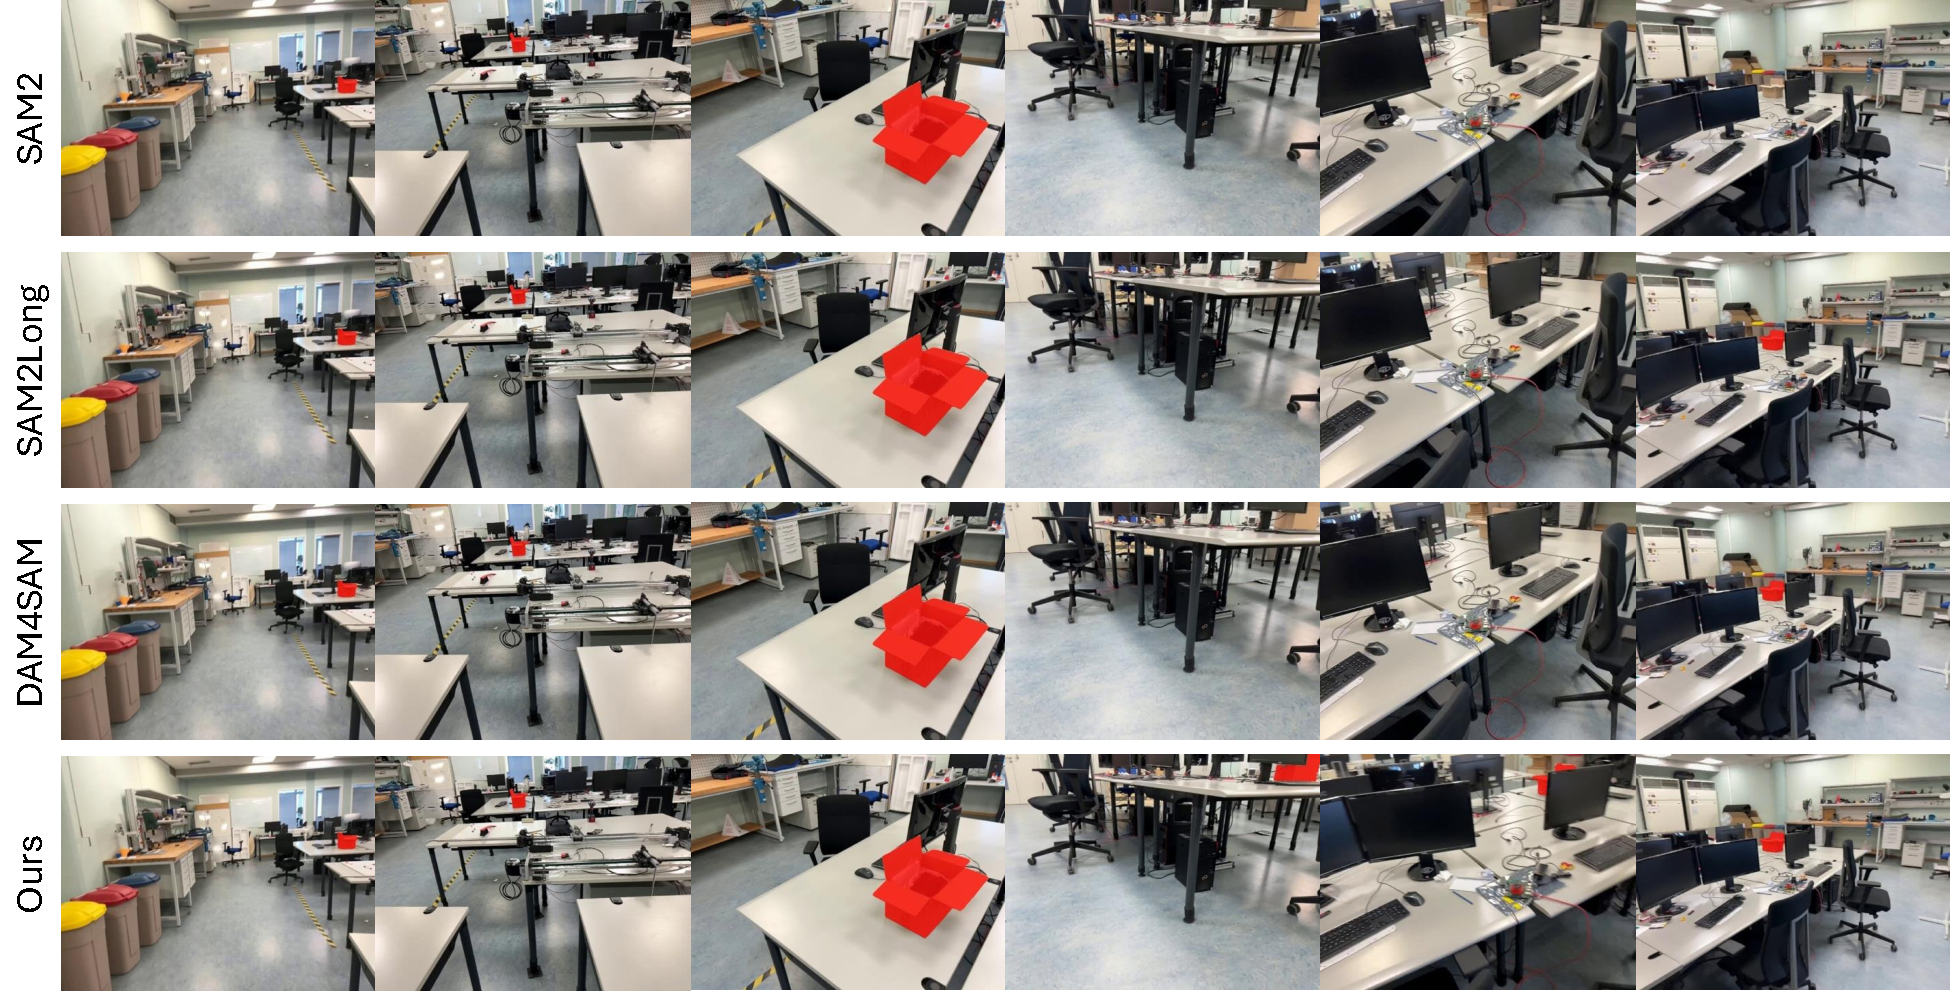
\includegraphics[width=1.0\textwidth]{figs/vis_comp.pdf}
    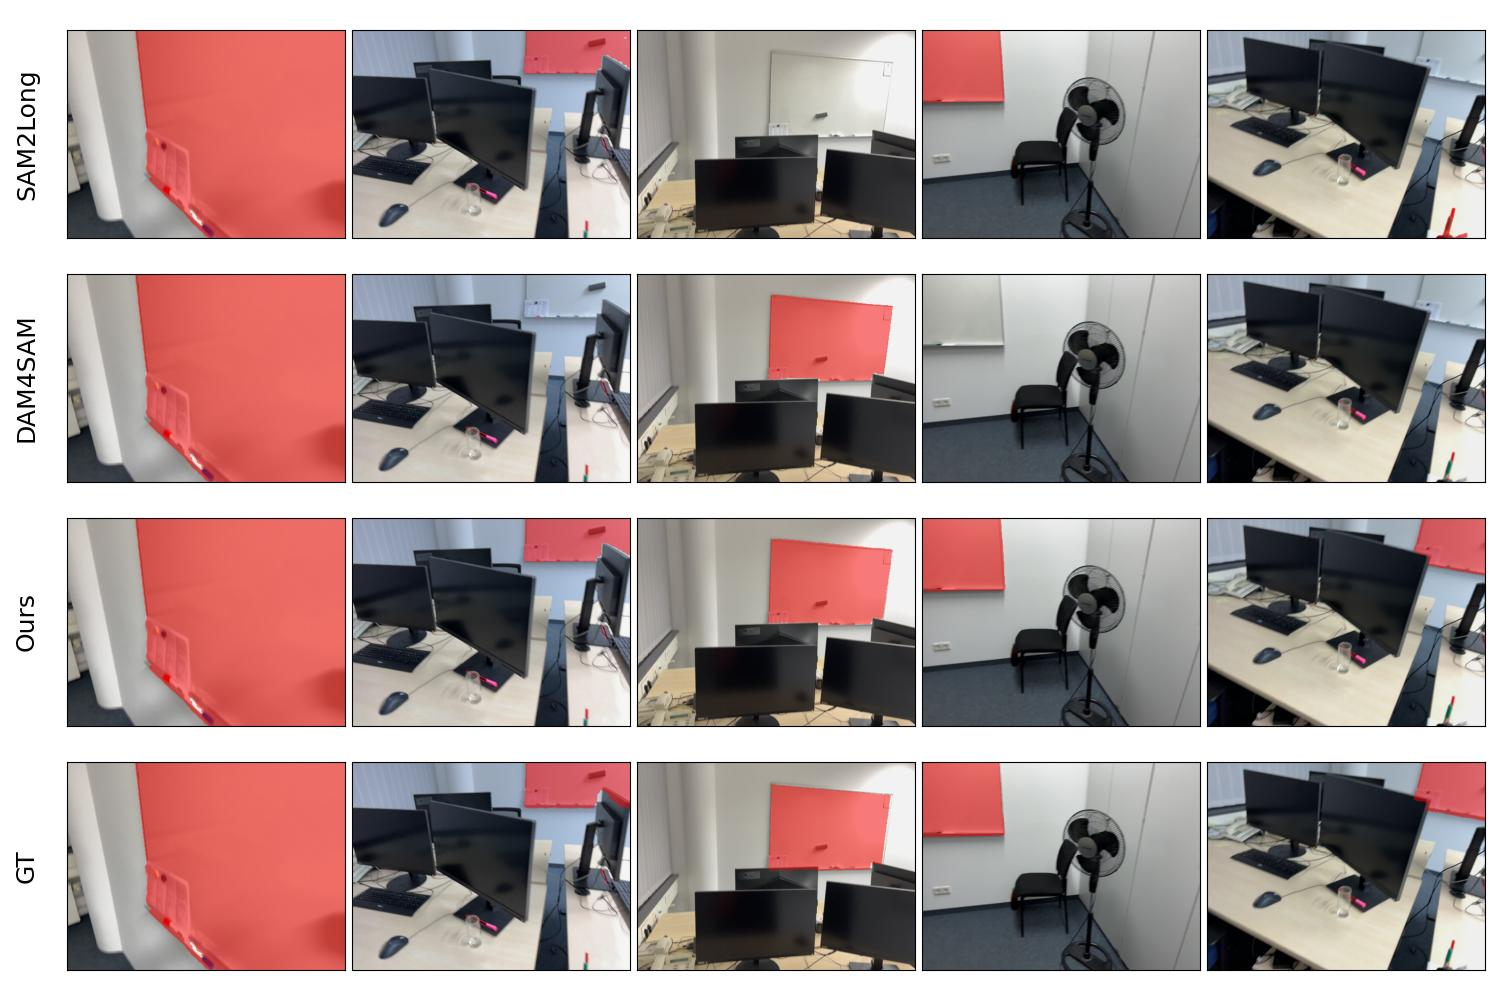
\includegraphics[width=1.0\textwidth]{figs/fig-vis/1ada7a0617/pred_masks_instance_512_7.jpg}
    \caption{
    \textbf{Visual comparison of different VOS methods}
    }
    \label{fig:vis_comp}
\end{figure*}

\begin{figure*}[t]
    \centering
    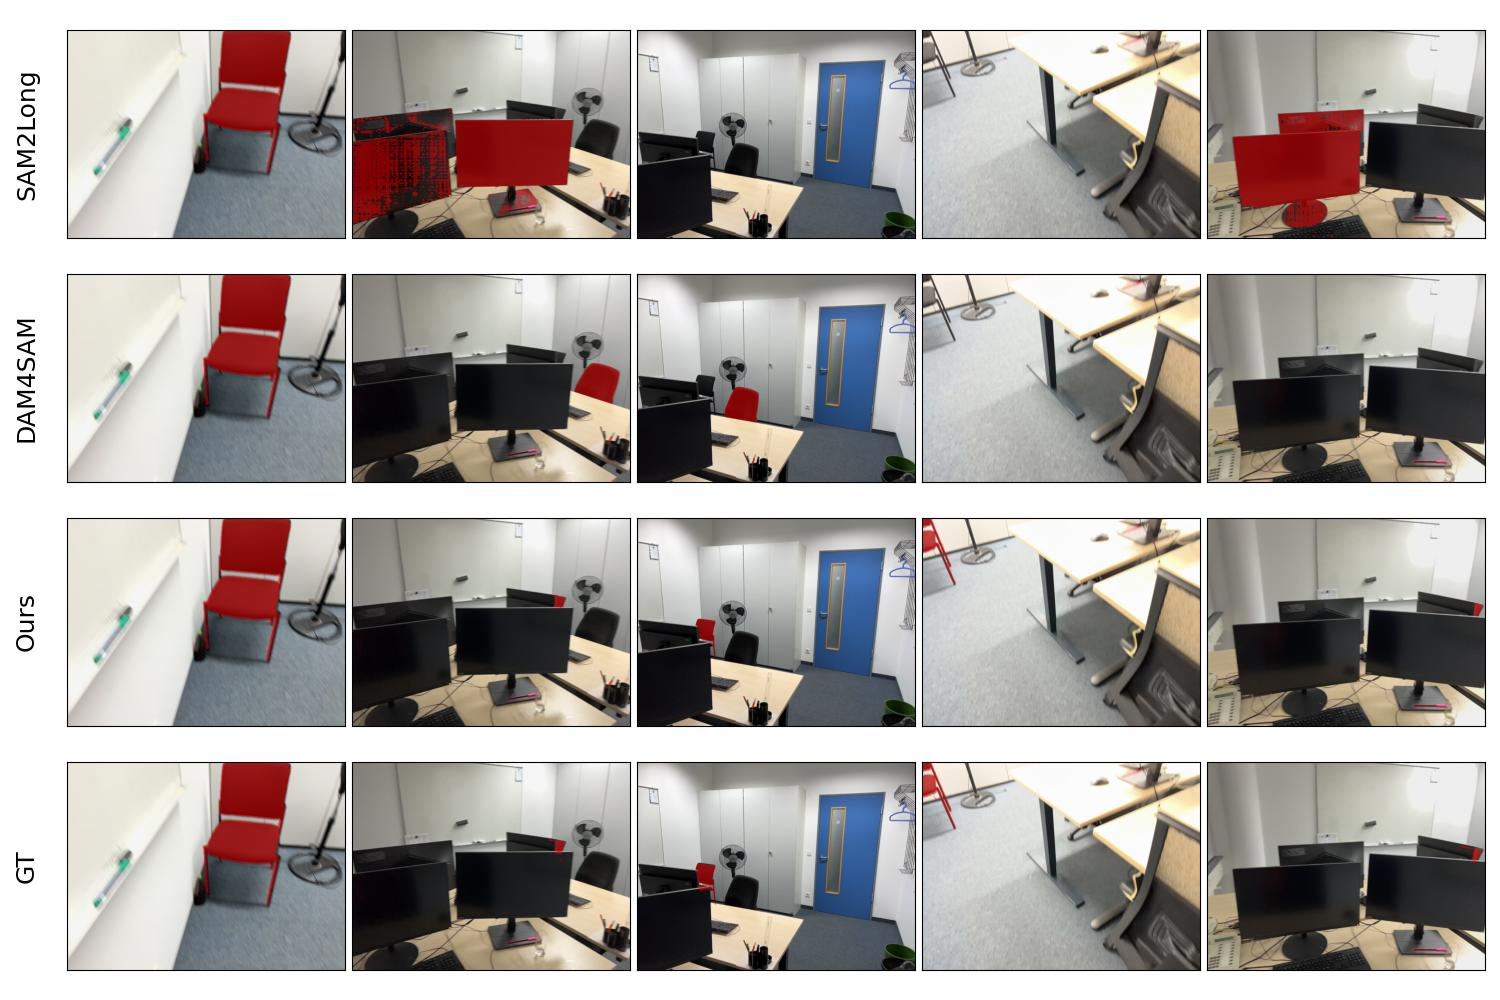
\includegraphics[width=1.0\textwidth]{figs/fig-vis/1ada7a0617/pred_masks_instance_512_11.jpg}
    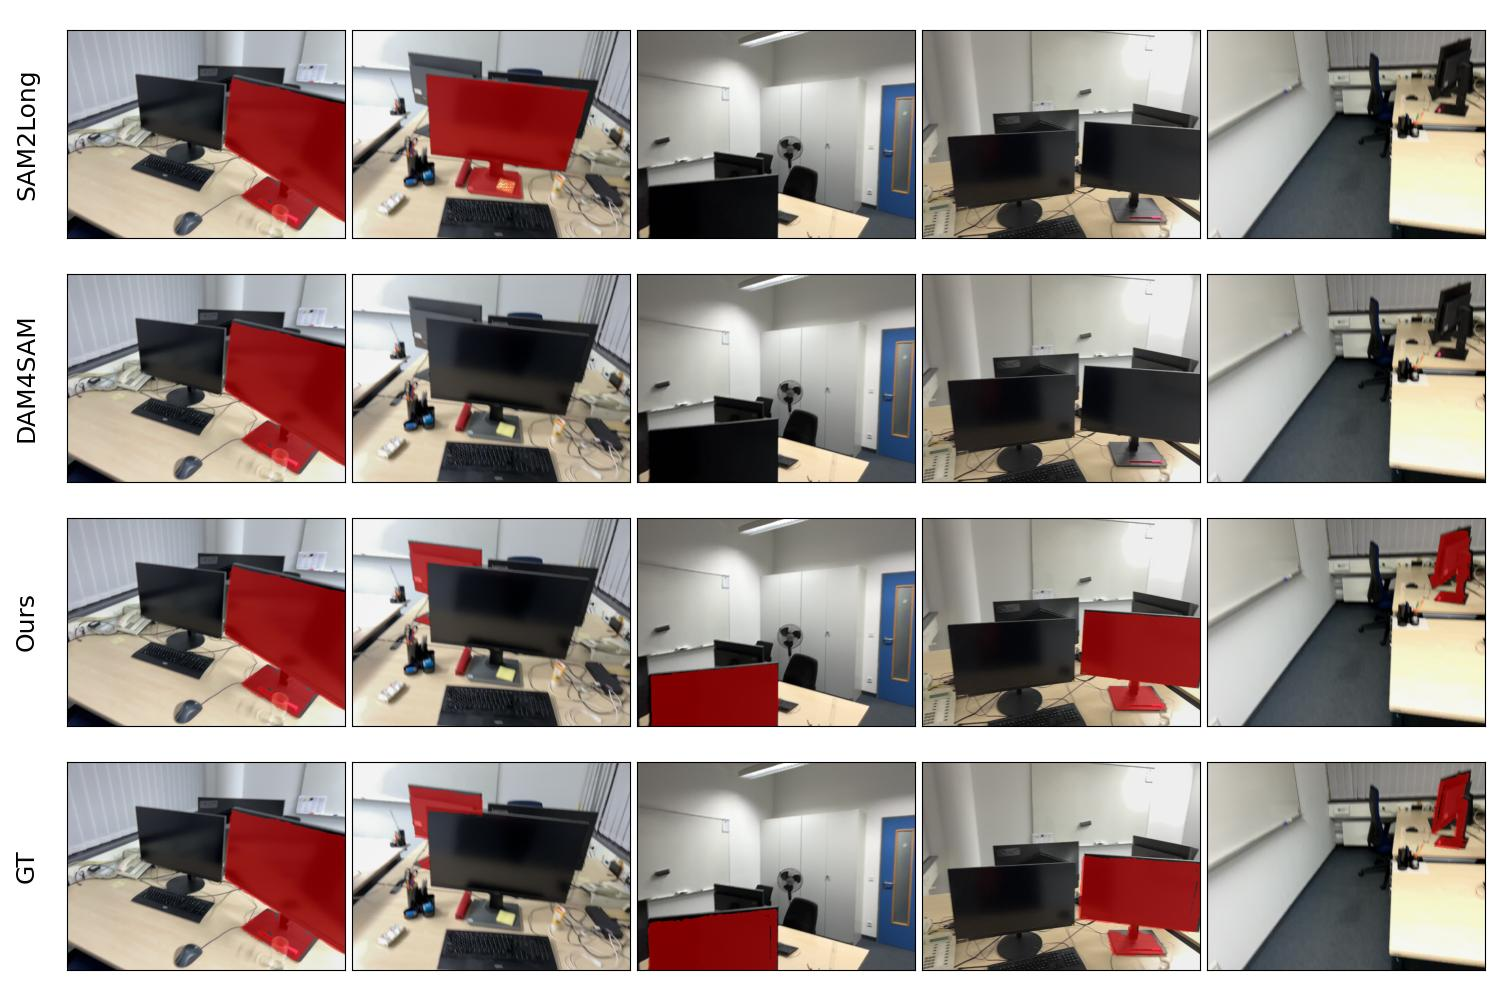
\includegraphics[width=1.0\textwidth]{figs/fig-vis/1ada7a0617/pred_masks_instance_512_36.jpg}
    \caption{
    \textbf{Visual comparison of different VOS methods}
    }
    \label{fig:vis_comp2}
\end{figure*}

\begin{figure*}[t]
    \centering
    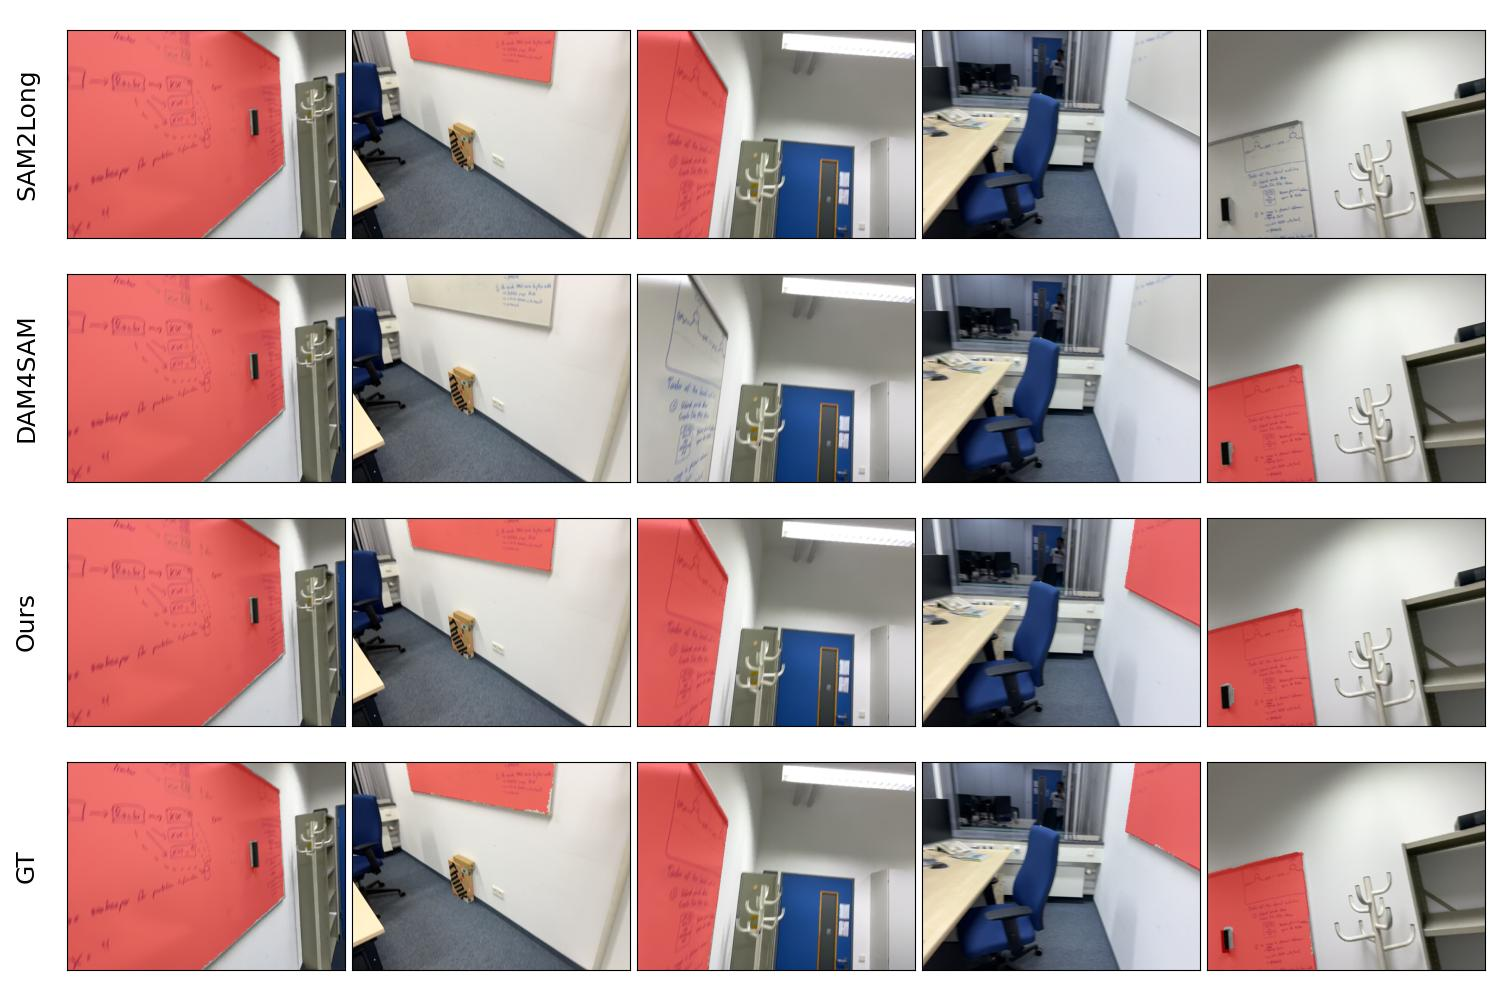
\includegraphics[width=1.0\textwidth]{figs/fig-vis/7b6477cb95/pred_masks_instance_512_10.jpg}
    
\includegraphics[width=1.0\textwidth]{figs/fig-vis/7b6477cb95/pred_masks_instance_512_11.jpg}
    \caption{
    \textbf{Visual comparison of different VOS methods}
    }
    \label{fig:vis_comp3}
\end{figure*}

\begin{figure*}[t]
    \centering
    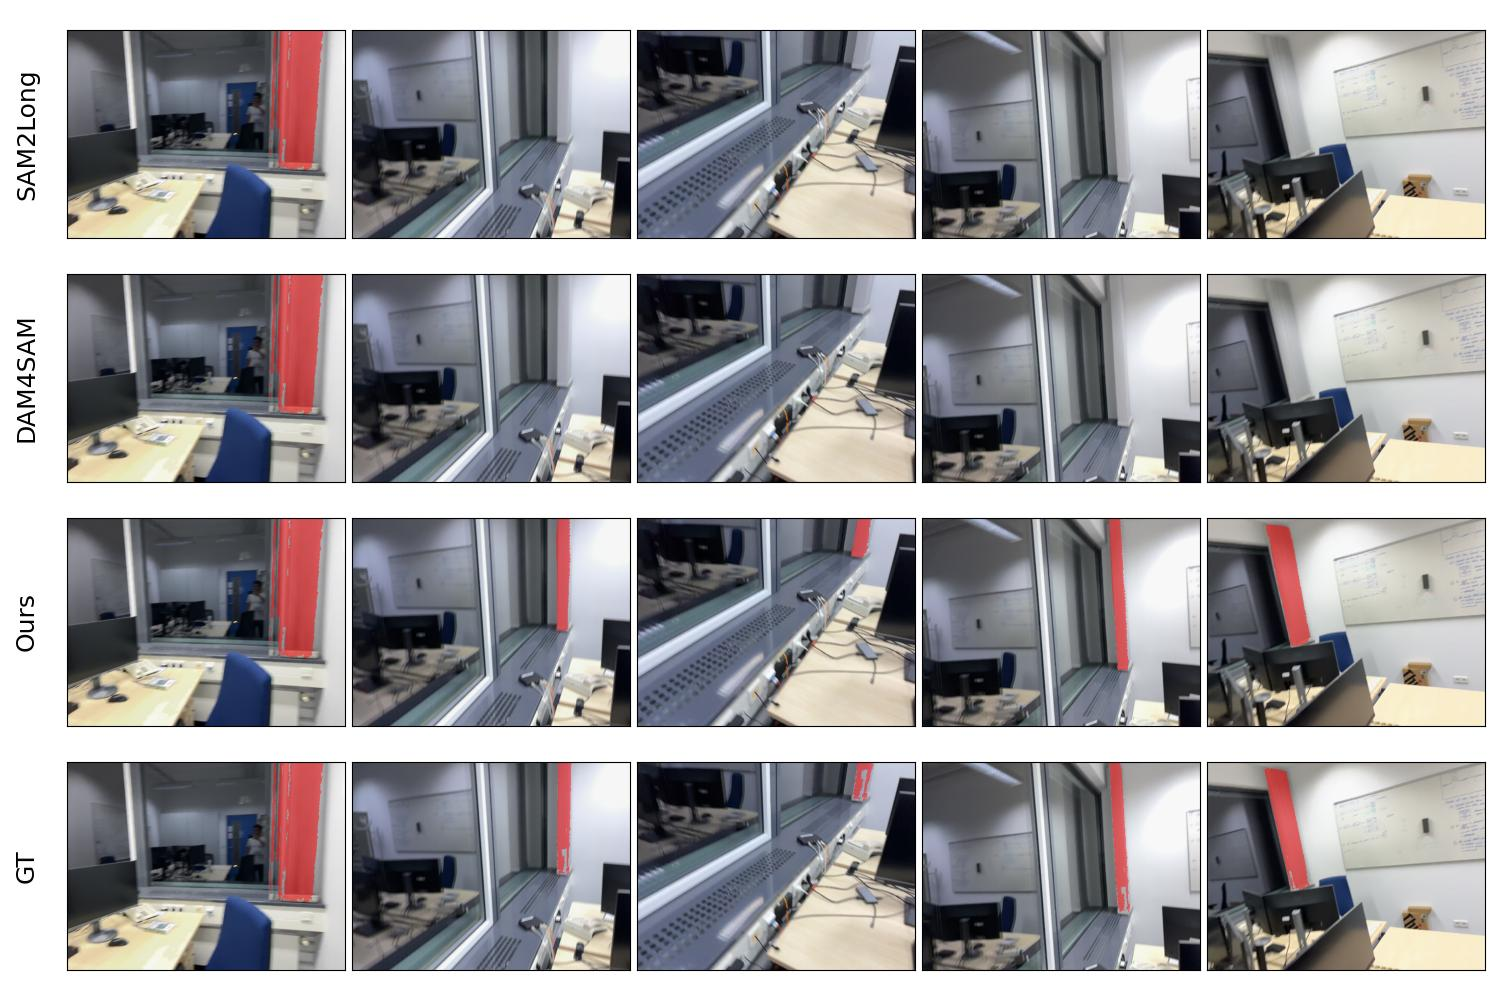
\includegraphics[width=1.0\textwidth]{figs/fig-vis/7b6477cb95/pred_masks_instance_512_45.jpg}
    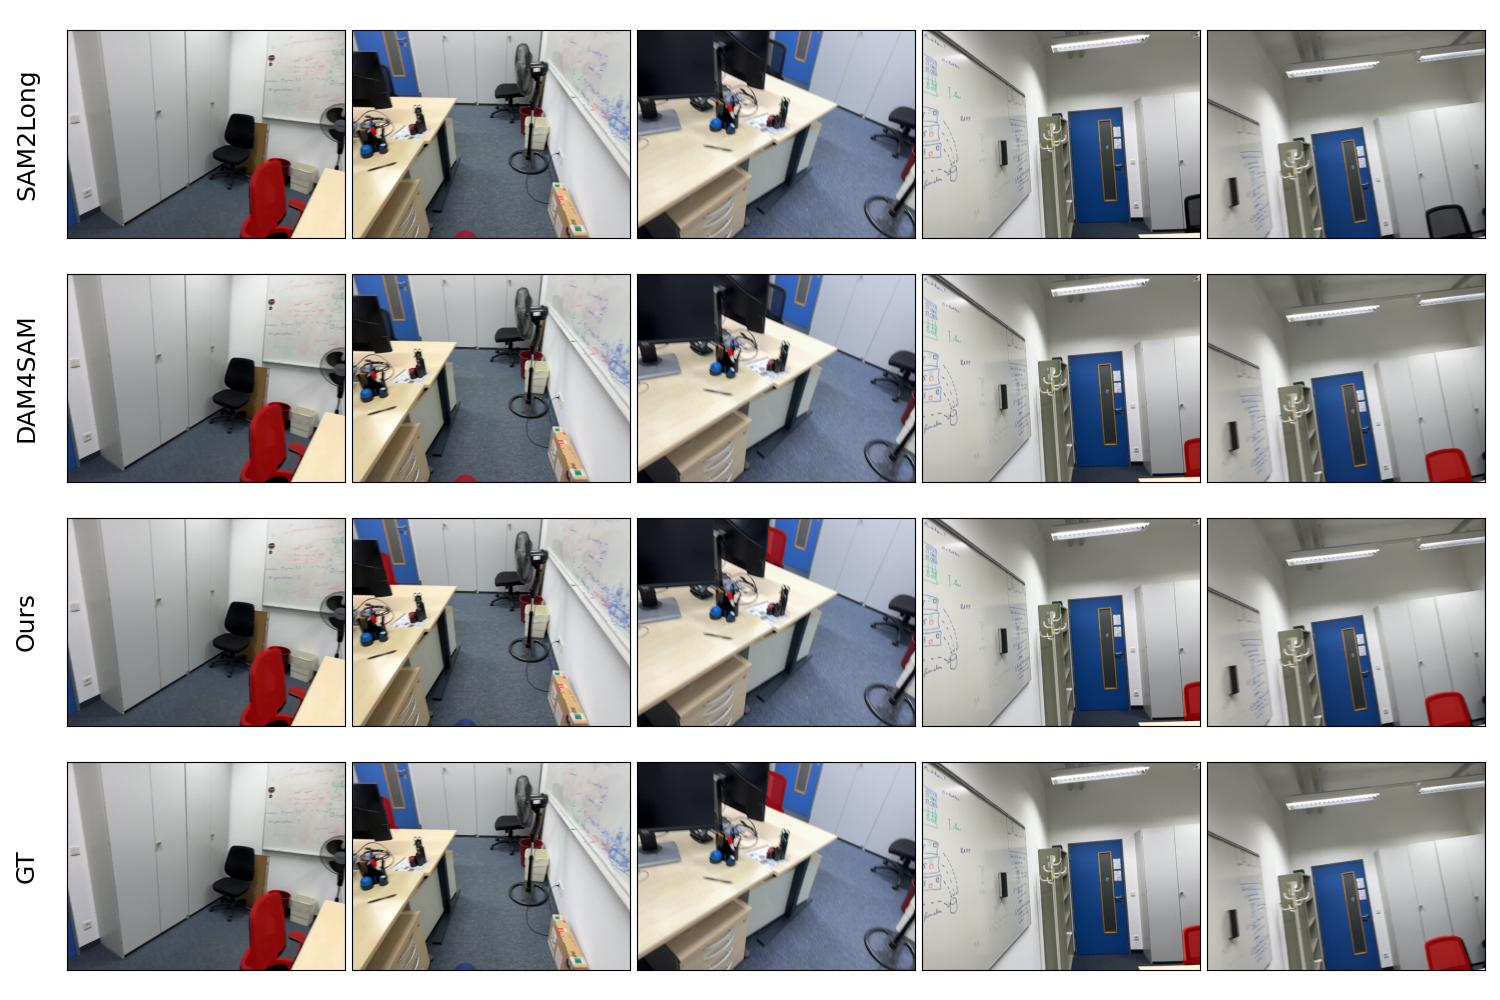
\includegraphics[width=1.0\textwidth]{figs/fig-vis/7b6477cb95/pred_masks_instance_512_53.jpg}
    \caption{
    \textbf{Visual comparison of different VOS methods}
    }
    \label{fig:vis_comp4}
\end{figure*}

\begin{figure*}[t]
    \centering
    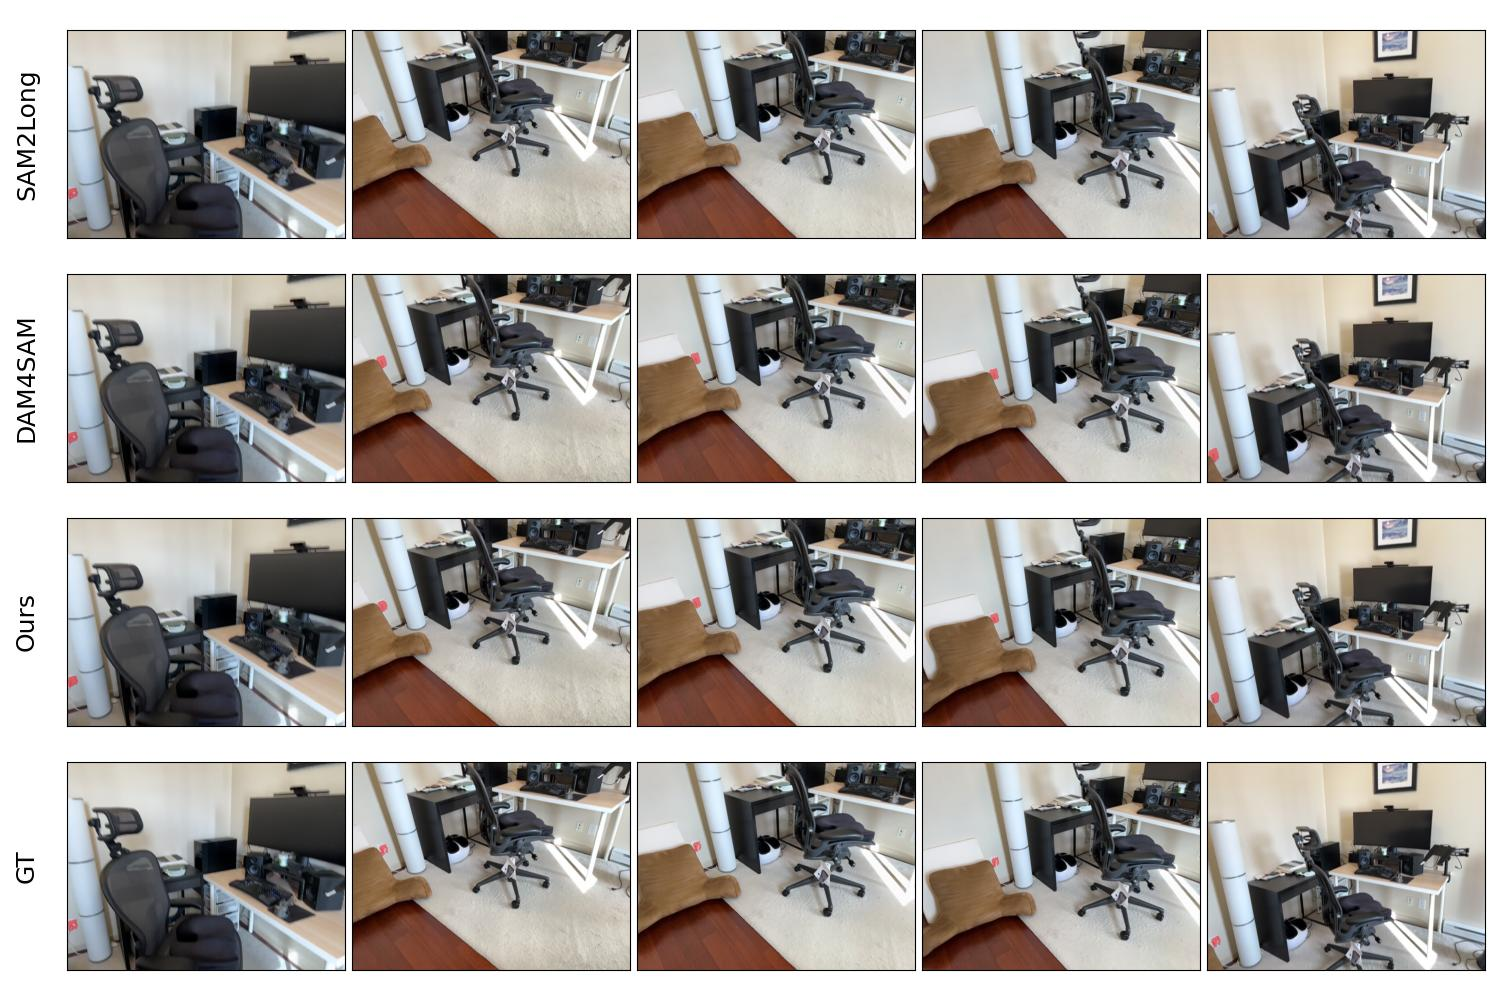
\includegraphics[width=1.0\textwidth]{figs/fig-vis/a24f64f7fb/pred_masks_instance_512_22.jpg}
    
\includegraphics[width=1.0\textwidth]{figs/fig-vis/acd95847c5/pred_masks_instance_512_10.jpg}
    \caption{
    \textbf{Visual comparison of different VOS methods}
    }
    \label{fig:vis_comp5}
\end{figure*}

\begin{figure*}[t]
    \centering
    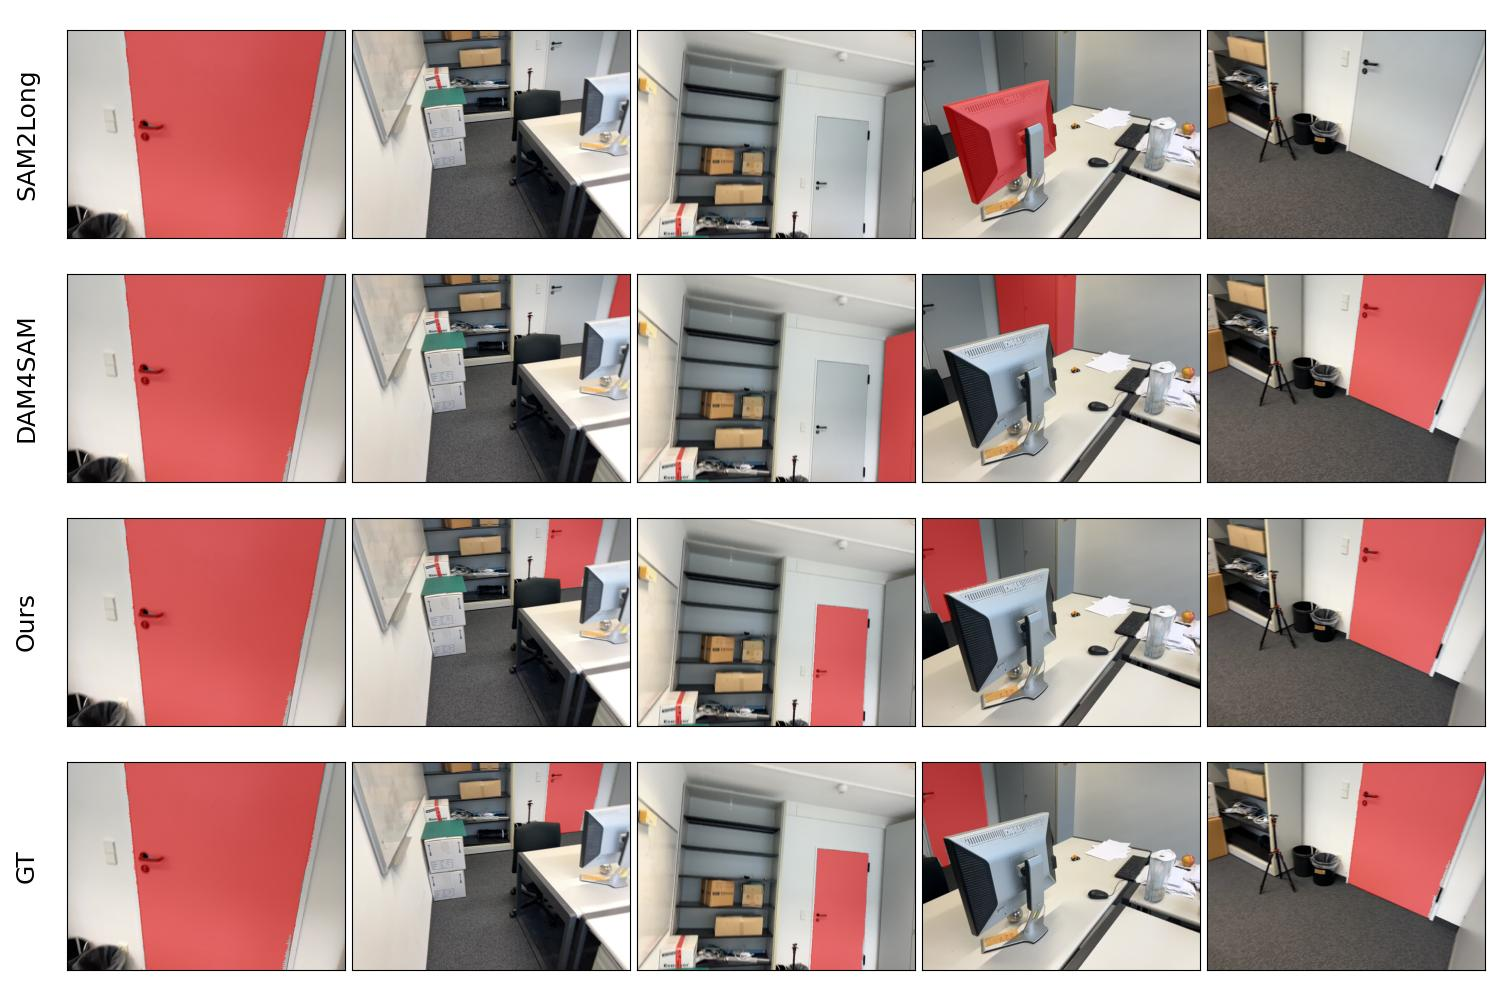
\includegraphics[width=1.0\textwidth]{figs/fig-vis/acd95847c5/pred_masks_instance_512_14.jpg}
    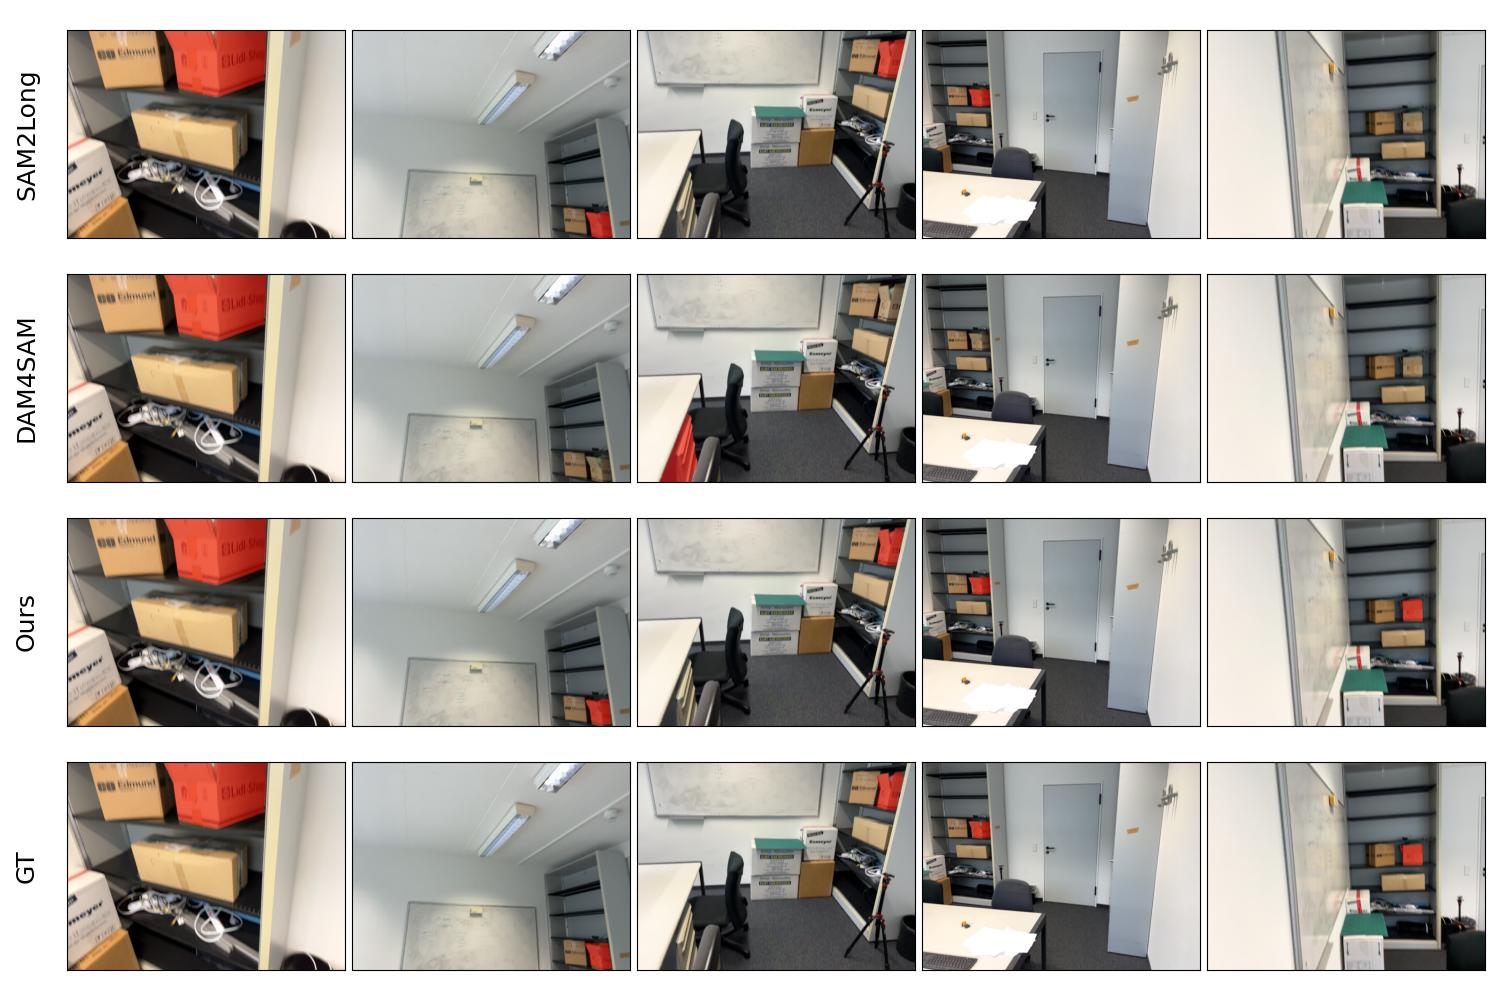
\includegraphics[width=1.0\textwidth]{figs/fig-vis/acd95847c5/pred_masks_instance_512_33.jpg}
    \caption{
    \textbf{Visual comparison of different VOS methods}
    }
    \label{fig:vis_comp6}
\end{figure*}

\begin{figure*}[t]
    \centering
    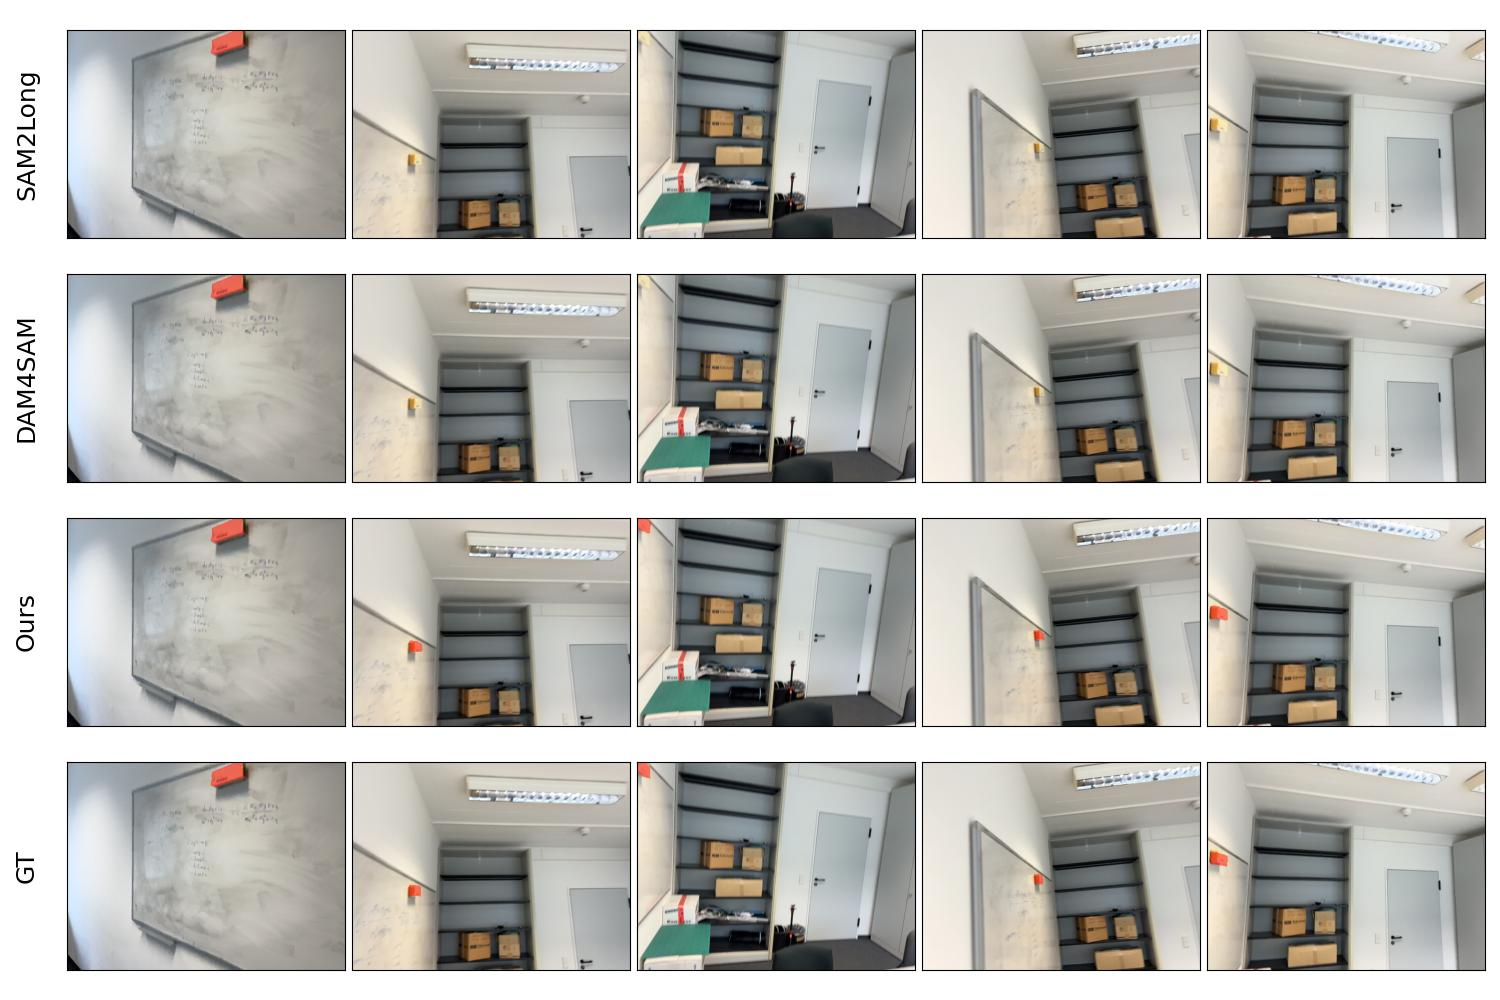
\includegraphics[width=1.0\textwidth]{figs/fig-vis/acd95847c5/pred_masks_instance_512_43.jpg}
    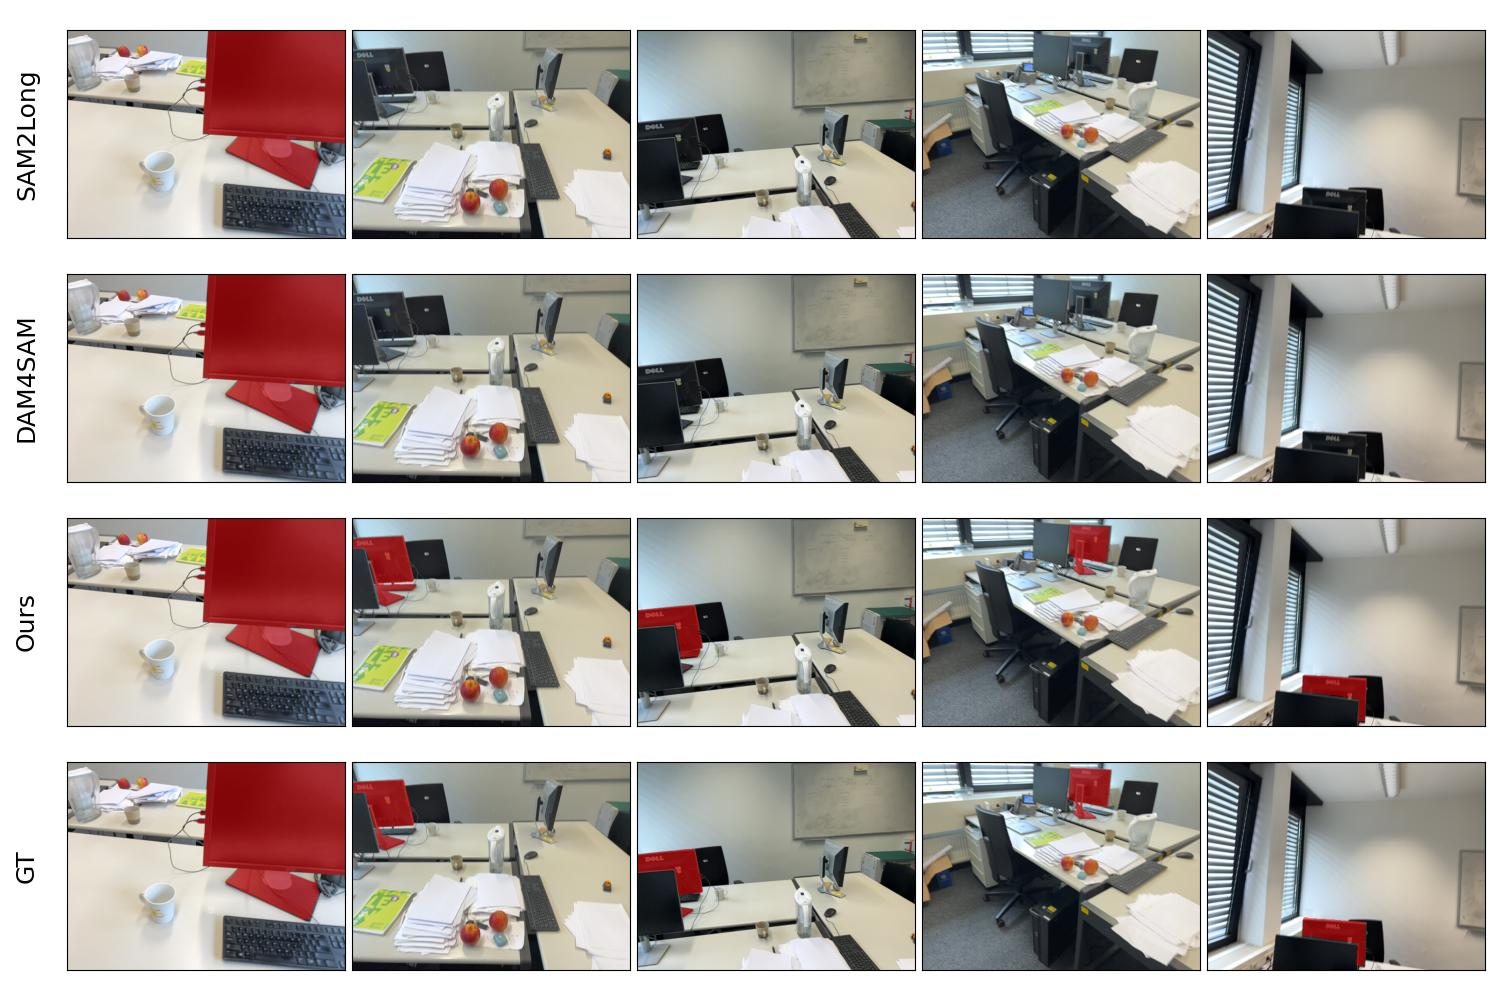
\includegraphics[width=1.0\textwidth]{figs/fig-vis/acd95847c5/pred_masks_instance_512_59.jpg}
    \caption{
    \textbf{Visual comparison of different VOS methods}
    }
    \label{fig:vis_comp7}
\end{figure*}

\section{Qualitative Comparison} \label{sec:more_qualitative}
\paragraph{Video Comparisoin}
We provide video object tracking visualization in \cref{fig:vis_comp,fig:vis_comp2,fig:vis_comp3,fig:vis_comp4,fig:vis_comp5,fig:vis_comp6,fig:vis_comp7}.
\paragraph{Class-Agnostic Instance Segmentation.}
We provide additional visual results on class-agnostic instance segmentation in~\cref{fig:visual_class}.




\begin{figure*}[ht]
\centering
\small
\setlength{\tabcolsep}{2pt}
% \renewcommand{\arraystretch}{1.0}
\resizebox{\textwidth}{!}{
\begin{tabular}{ccc}
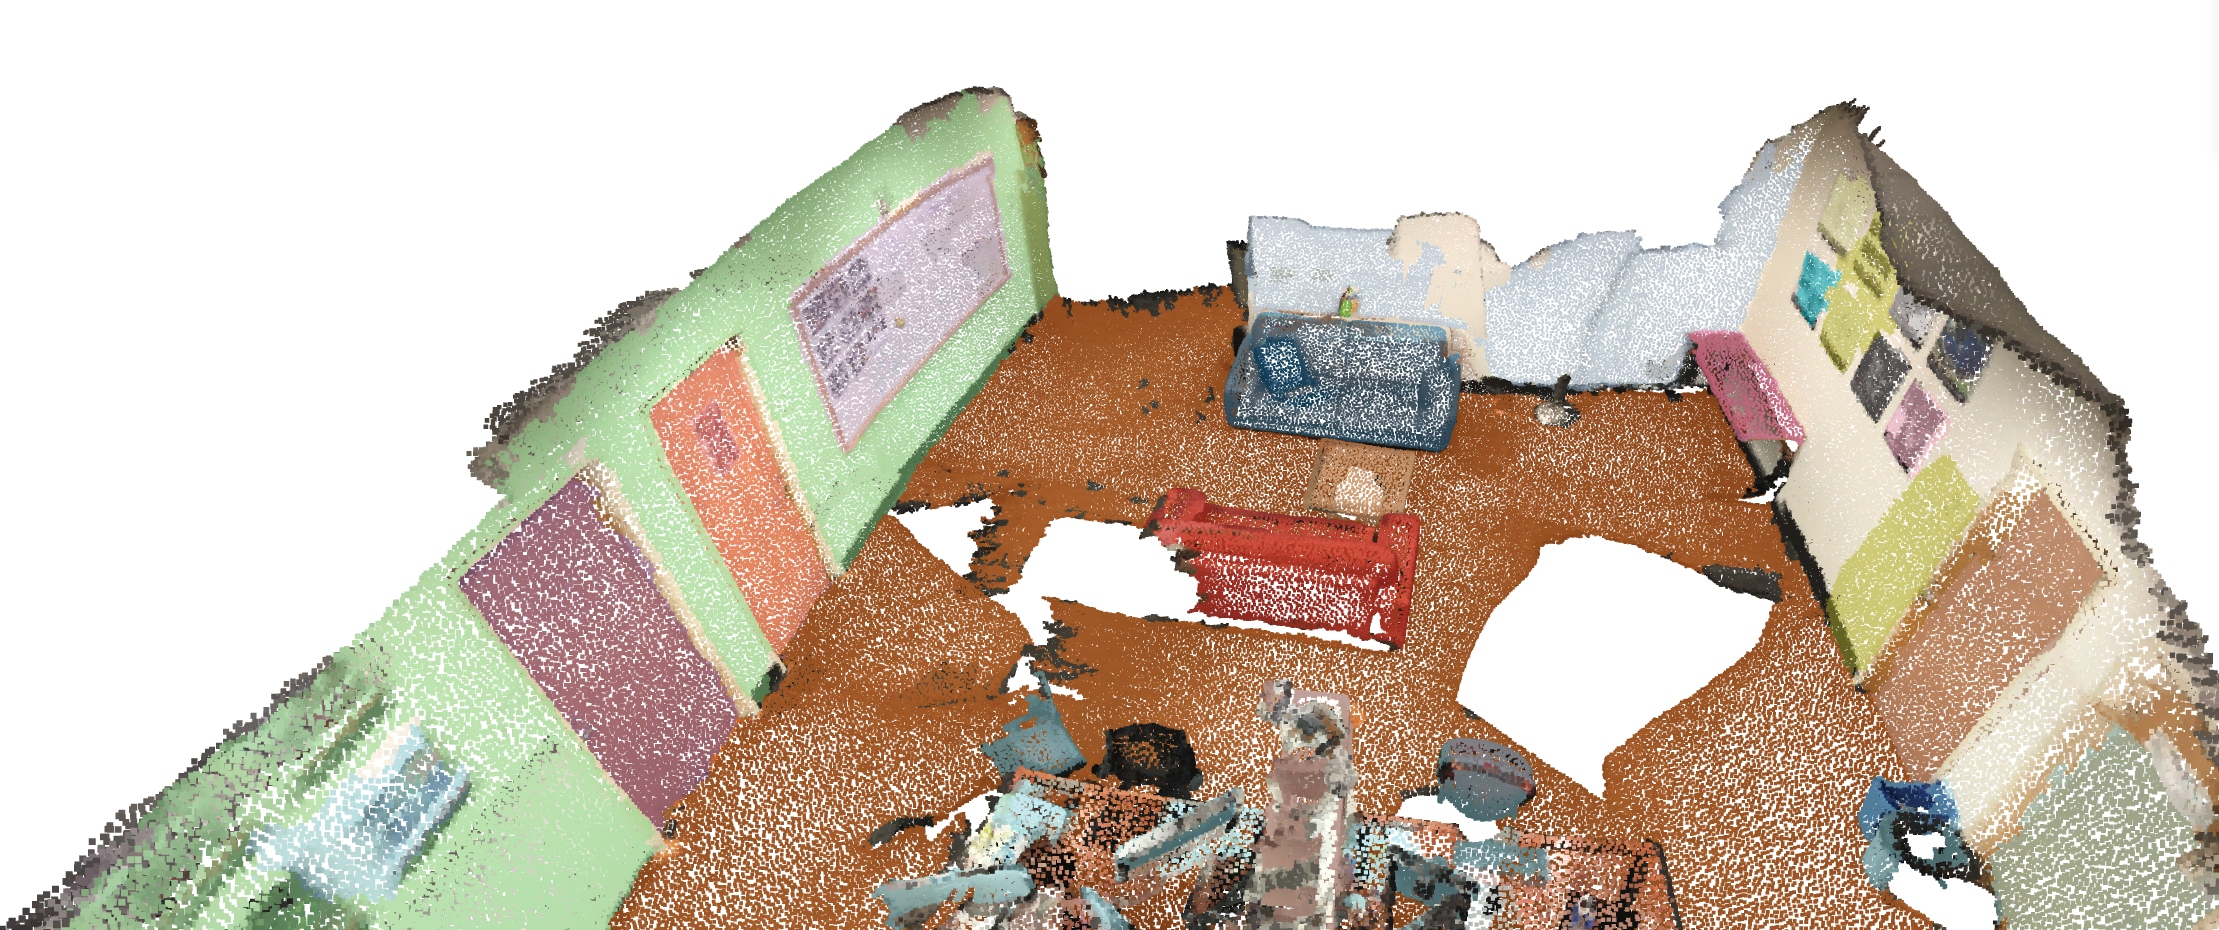
\includegraphics[width=0.33\textwidth]{figs/3D-Visual/1_1.png} & 
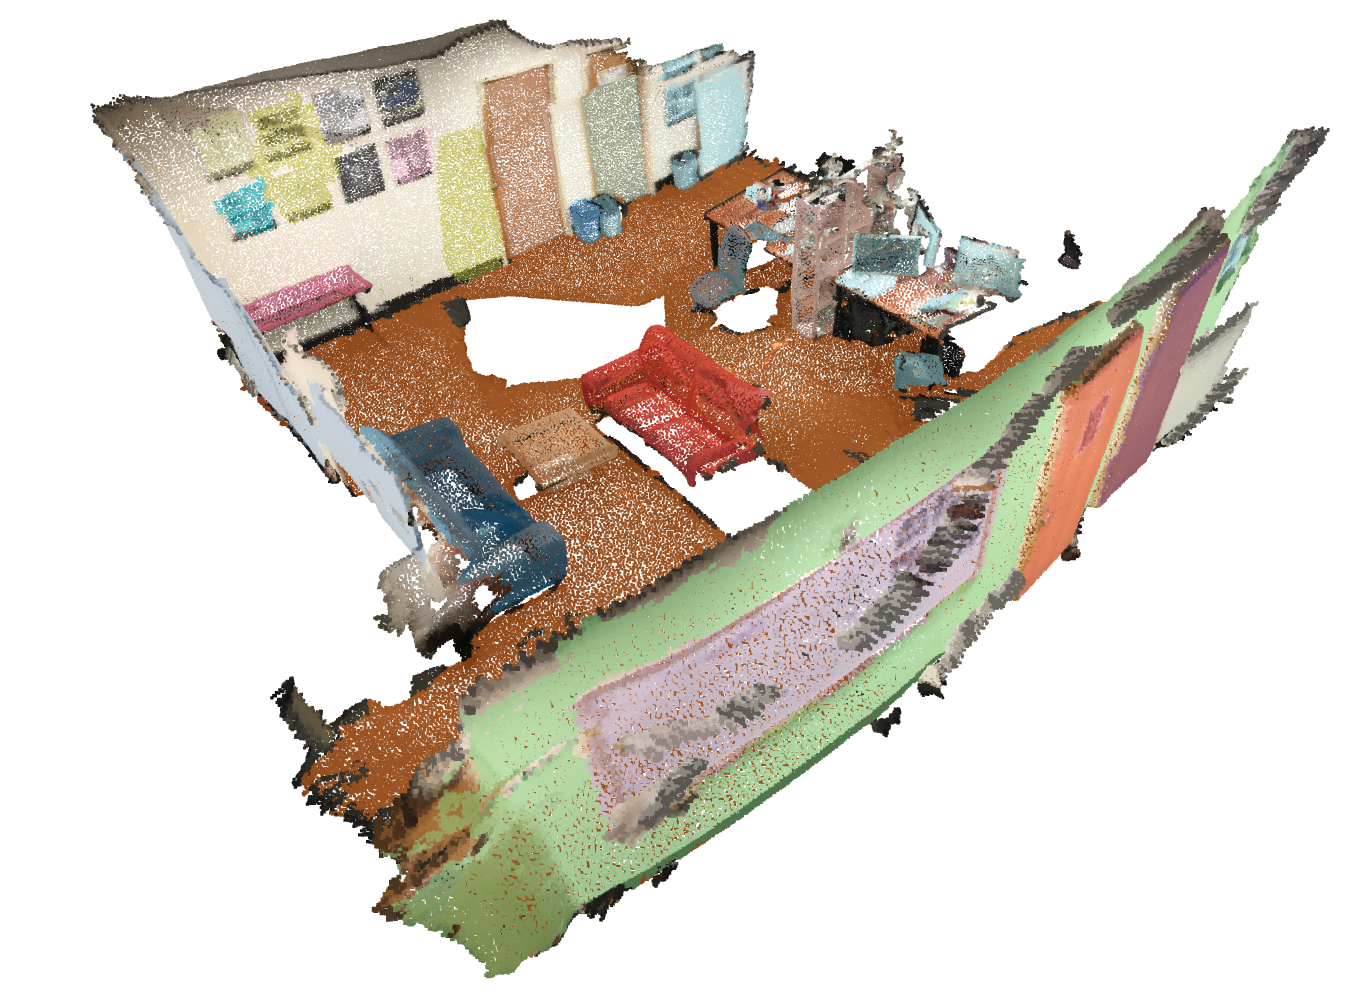
\includegraphics[width=0.33\textwidth]{figs/3D-Visual/1_2.png} & 
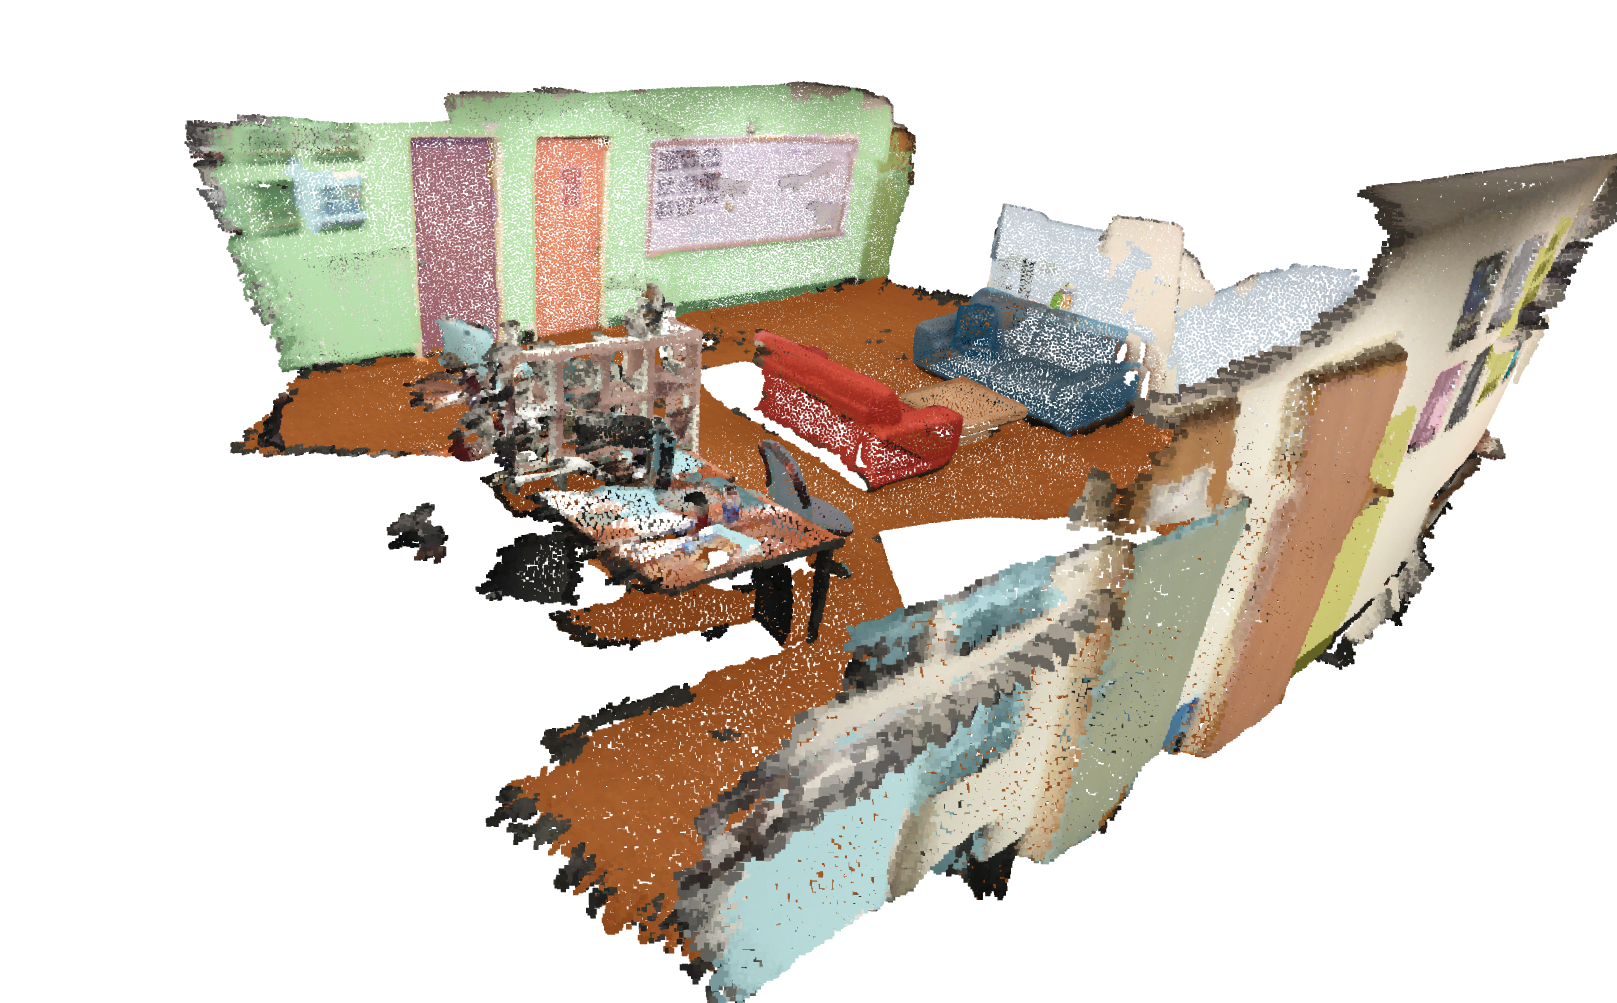
\includegraphics[width=0.33\textwidth]{figs/3D-Visual/1_3.png} \\
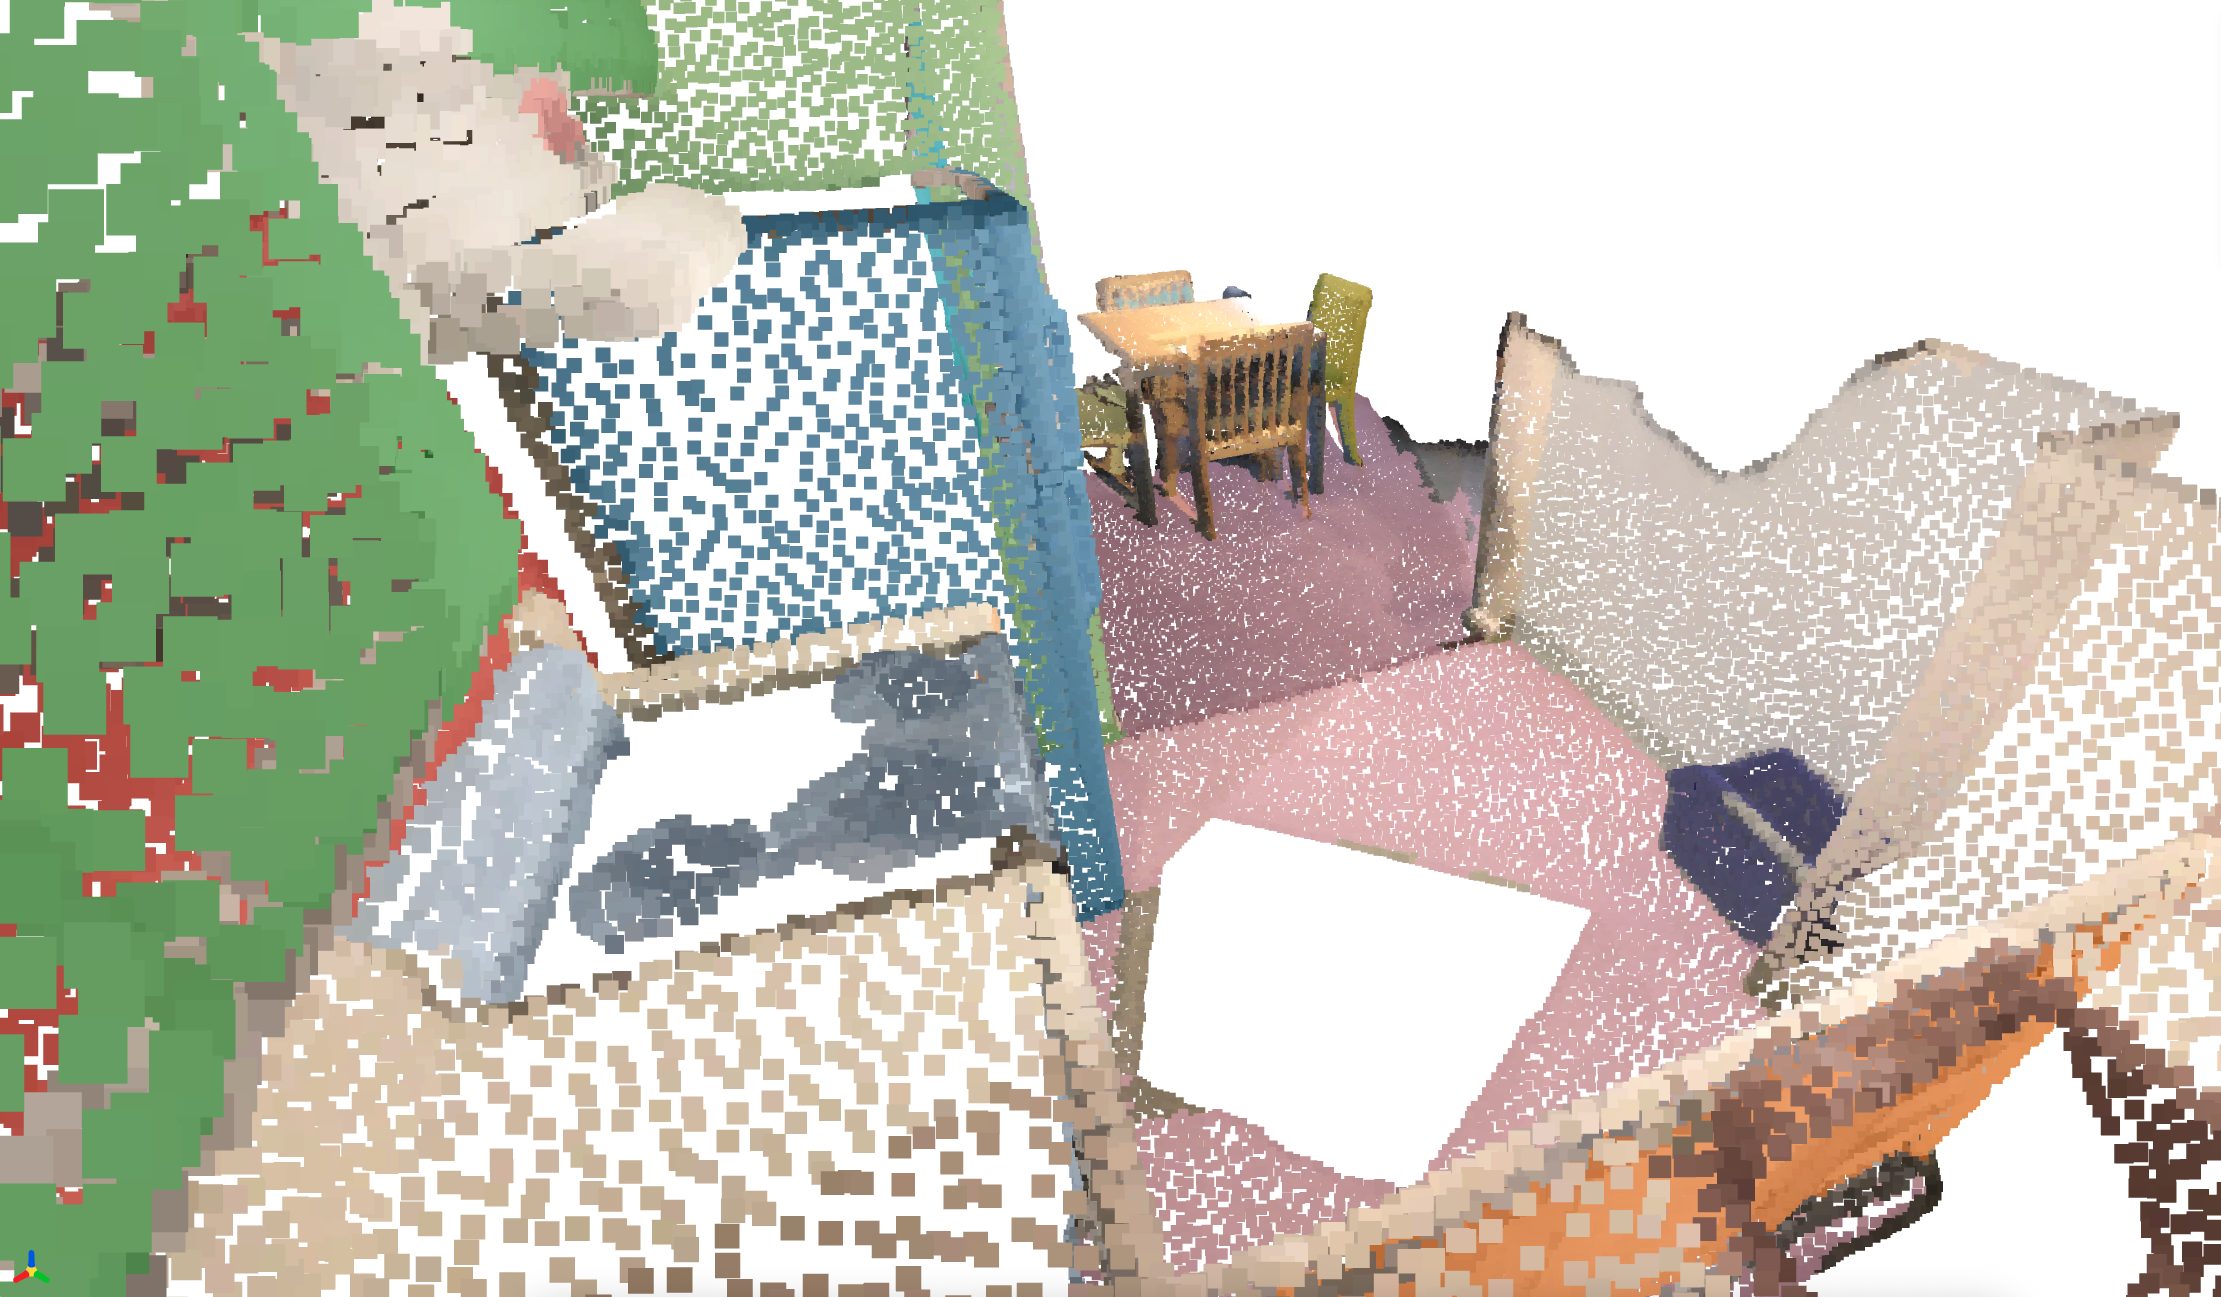
\includegraphics[width=0.33\textwidth]{figs/3D-Visual/2_1.png} & 
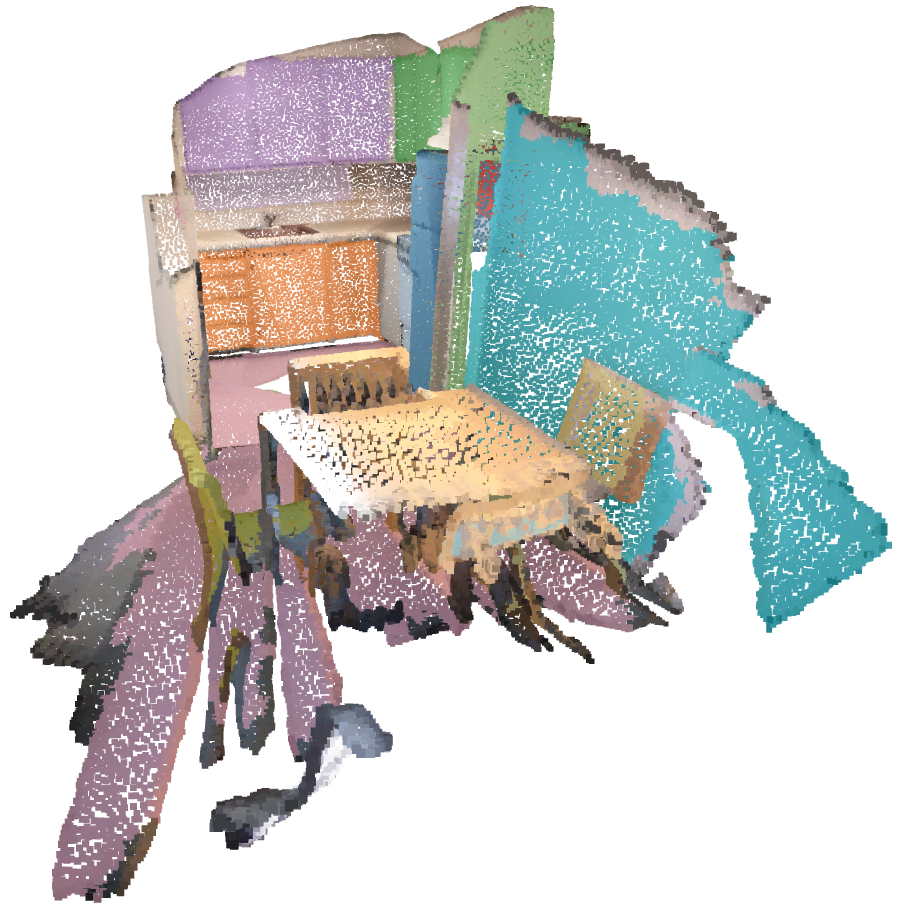
\includegraphics[width=0.33\textwidth]{figs/3D-Visual/2_2.png} & 
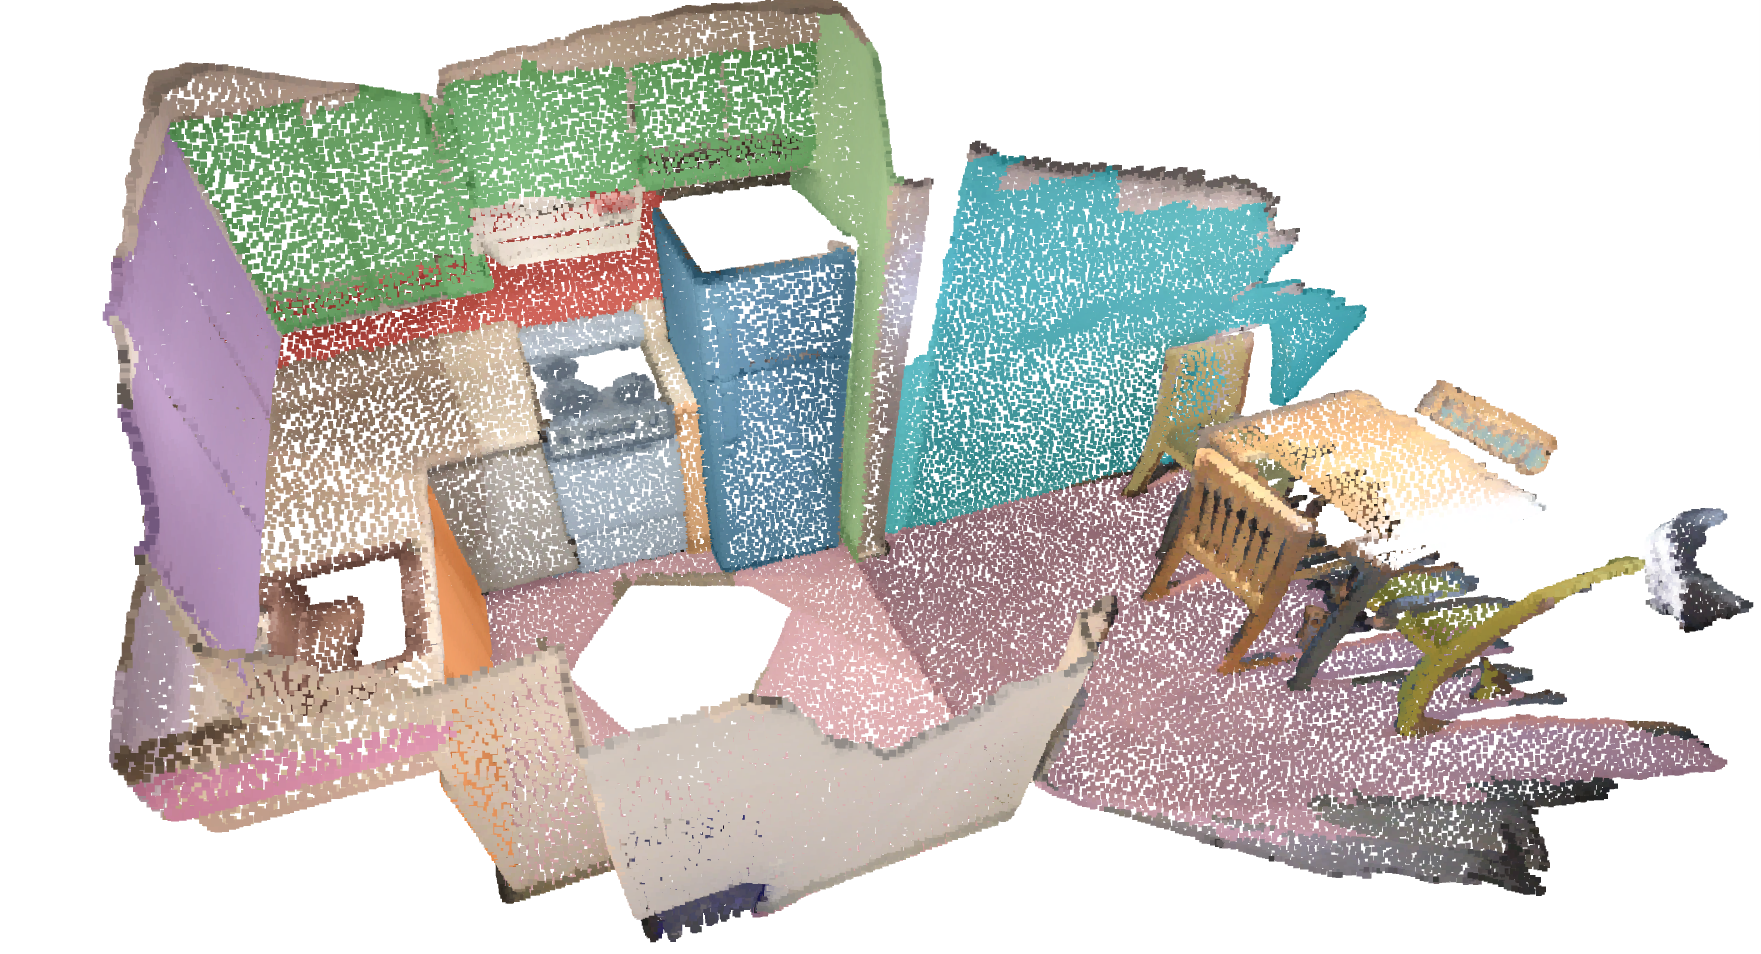
\includegraphics[width=0.33\textwidth]{figs/3D-Visual/2_3.png} \\
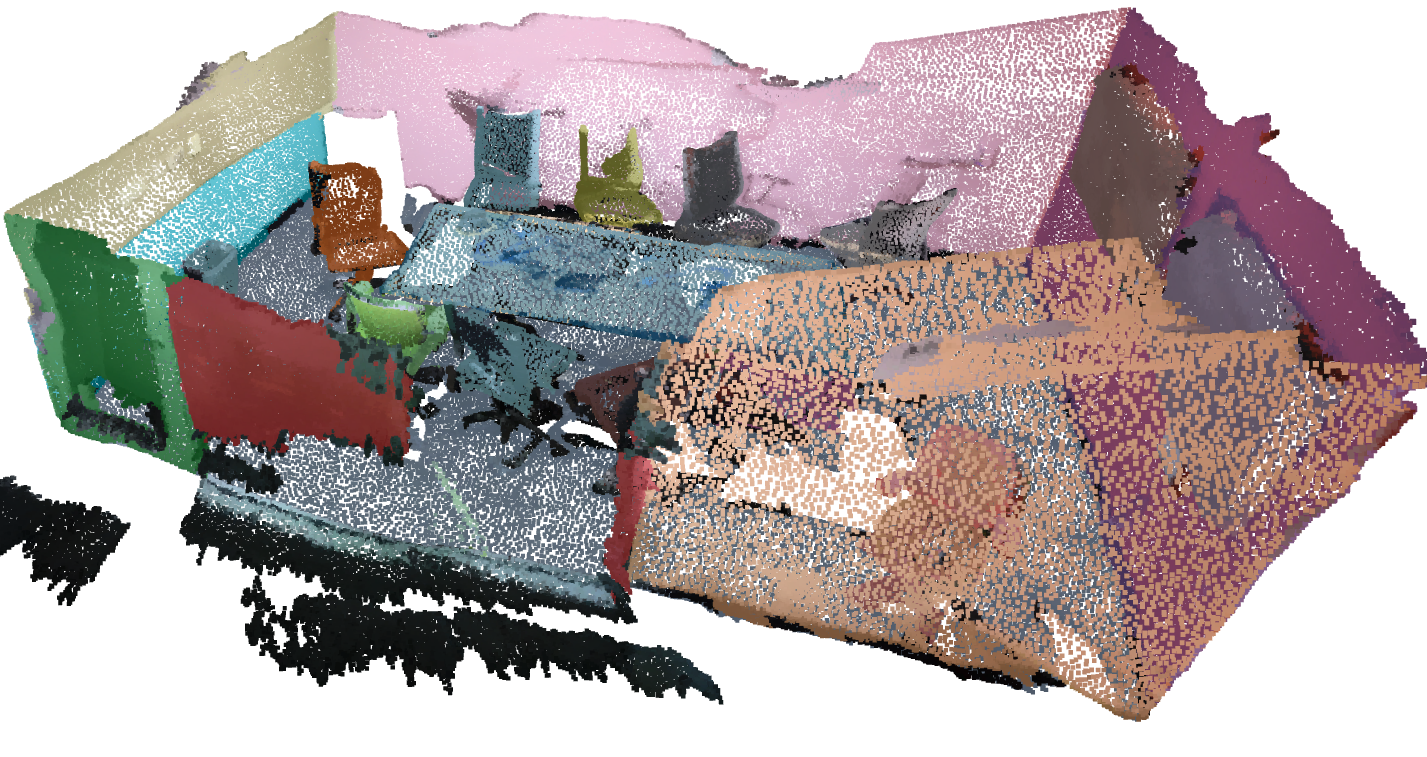
\includegraphics[width=0.33\textwidth]{figs/3D-Visual/3_1.png} & 
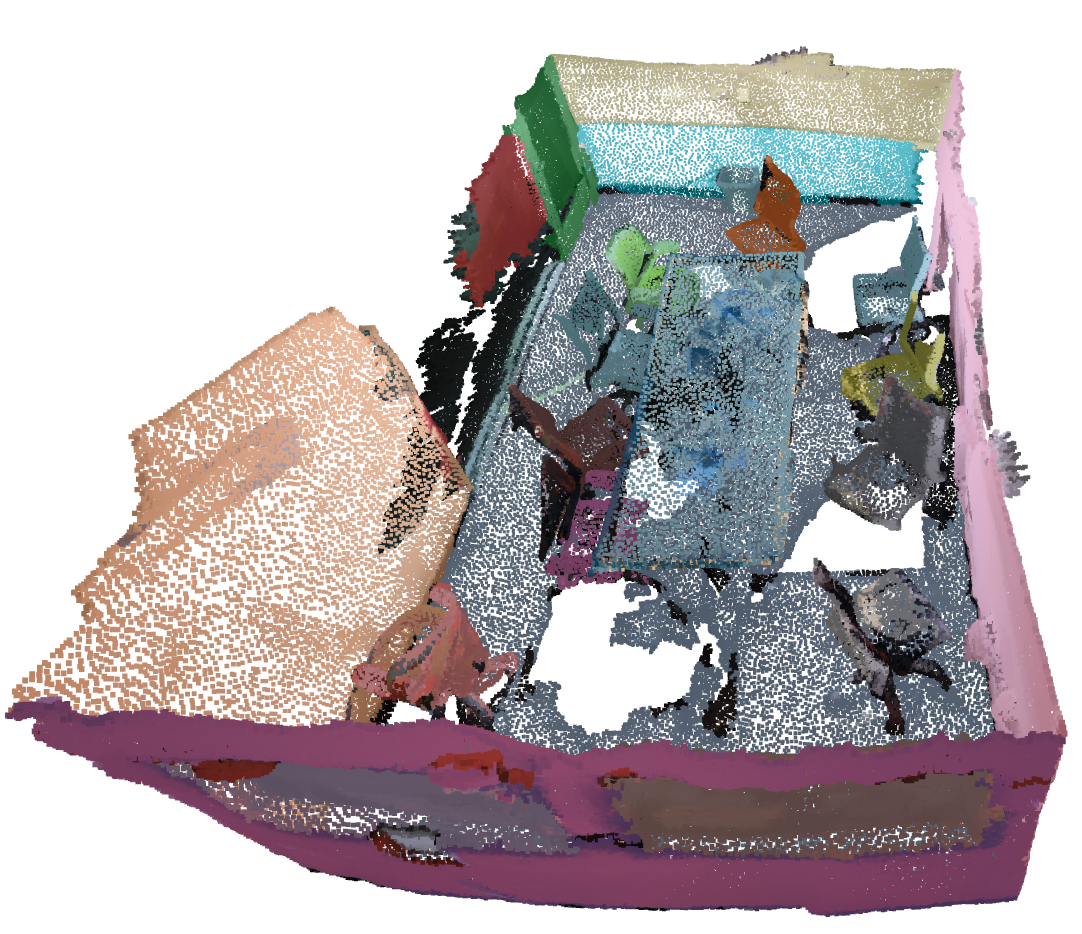
\includegraphics[width=0.33\textwidth]{figs/3D-Visual/3_2.png} & 
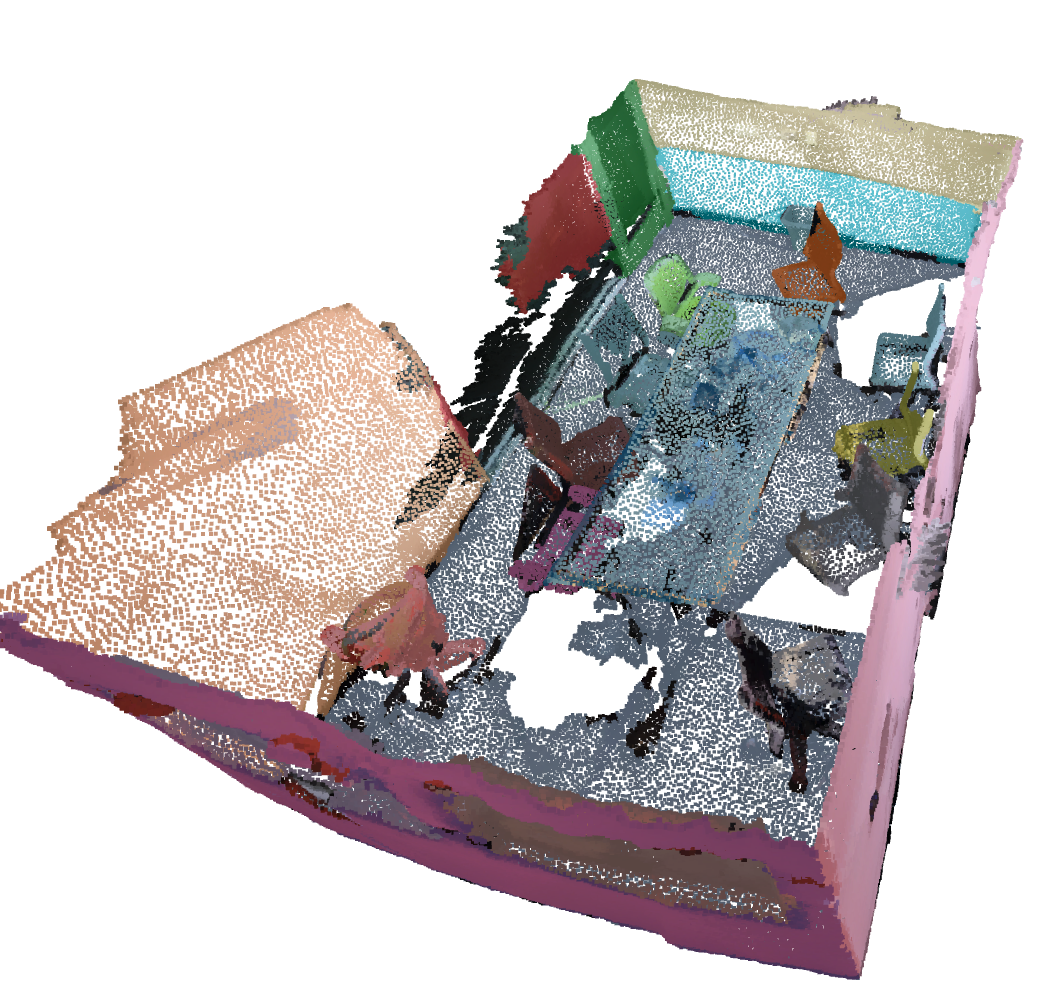
\includegraphics[width=0.33\textwidth]{figs/3D-Visual/3_3.png} \\
\end{tabular}
}
\caption{
\textbf{Visual results on class-agnostic instance segmentation.}
}
\label{fig:visual_class}
\end{figure*}
